\section{Sistemi di Comunicazione}
    Un sistema di comunicazione numerico puó essere approssimato a
    \begin{figure}[H]
        \centering 
        \begin{tikzpicture}[
            node distance=3cm,
            >=latex
            ]

            \node [coordinate] (input) {};
            \node [draw, rectangle,right of = input, minimum height=3em, minimum width=6em] (block) {$\substack{\text{Sistema di} \\ \text{Comunicazione Numerico}}$};
            \node [coordinate, right of = block] (output) {};
            
            \draw[draw,->] (input) --node[above]{$\{b_n$\}} (block);
            \draw[->] (block) --node[above]{$\{\hat{b}_n$\}} (output);
        \end{tikzpicture}    
    \label{sistema di comunicazione numerico}
    \end{figure}
    Dove all'interno del sistema sono racchiusi il Trasmettitore ($Tx$), il canale di trasmissione ($c$) e il Ricevitore ($Rx$).
    il sistema prende in ingresso dei bit, o un segnale analogico opportunamente nuemrizzato, e li trasmette su di un canale numerico inviandoli ad un ricevitore.
    Analizziamo la parte di trasmissione:
    \begin{figure}[H]
        \centering
            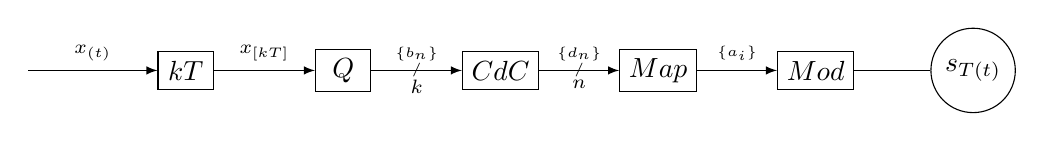
\begin{tikzpicture}[
                    node distance=2cm,
                    >=latex
                ]
                % Blocks
                \node [coordinate] (input) {};
                \node [rectangle, draw,minimum height=1em, minimum width=2em,right of=input] (AD) {$kT$};
                \node [rectangle, draw,minimum height=1em, minimum width=2em,right of=AD] (Q) {$Q$};
                \node [rectangle, draw,minimum height=1em, minimum width=2em,right of=Q] (CS) {$CdC$};
                \node [rectangle, draw,minimum height=1em, minimum width=2em,right of=CS] (CC) {$Map$};
                \node [rectangle, draw,minimum height=1em, minimum width=2em,right of=CC] (TX) {$Mod$};
                \node [circle,draw,right of=TX] (TXant) {$s_{T(t)}$};
            
                % Connections
                \draw [->] (input) --node[above]{\scriptsize$x_{(t)}$} (AD);
                \draw [->] (AD) --node[above]{\scriptsize$x_{[kT]}$} (Q);
                \draw [->] (Q) --node[above]{\tiny$\{b_n\}$}node[midway]{\tiny$/$} node[below]{\scriptsize$k$} (CS);
                \draw [->] (CS) --node[above]{\tiny$\{d_n\}$}node[midway]{\tiny$/$} node[below]{\scriptsize$n$} (CC);
                \draw [->] (CC) --node[above]{\tiny$\{a_i\}$} (TX);
                \draw [-] (TX) -- (TXant);
            \end{tikzpicture}    
        \label{fig:Sistema di comunicazione numerico trasmettitore}
        \caption{Esempio sistema di trasmettitore}
    \end{figure}
    \begin{itemize}
        \item {CdC: Codifica di Canale, si occupa di aggiungere ridondanza ai bit in ingresso per proteggerli da eventuali errori del canale di trasmissione ho di
            conseguenza che $k<n$, puó essere preceduto da un eventuale codifica di sorgente. 
            \begin{figure}[H]
                \centering 
                \begin{tikzpicture}[
                    node distance=3cm,
                    >=latex
                    ]
        
                    \node [coordinate] (input) {};
                    \node [draw, rectangle,right of = input, minimum height=3em, minimum width=6em] (block) {$\substack{\text{Codifica di} \\ \text{Canale}}$};
                    \node [coordinate, right of = block] (output) {};
                    
                    \draw[draw,->] (input) --node[above]{$\{b_n$\}} node[midway]{\tiny$/$} node[below]{\scriptsize$k,R_b$}(block);
                    \draw[->] (block) --node[above]{$\{d_n$\}} node[midway]{\tiny$/$} node[below]{\scriptsize$n,R_d$} (output);
                \end{tikzpicture}    
            \end{figure}
            $R_b = \frac{1}{T_b}$ é il Bit Rate a cui i bit sono generati in ingresso mentre, $R_d = \frac{1}{T_d}$ é il Bit Rate di uscita. Volendo trvare la relazione tra ingresso e uscita:
            \[
                kT_b = nT_d \Rightarrow \frac{R_b}{R_d} = \frac{k}{n}     
            \] 
            il quale é compreso tra $0<\frac{R_b}{R_d}\leq 1$ se cosí non fosse non introdurrei ridondanza, il rate in ingresso deve essere inferiore a quello di uscita o non 
            potrei introdurre bit aggiuntivi.
        }
        \item {Map: Mappatore ($M$), trasforma una \emph{sequenza} di bit di codice $\{d_n\}$ in una sequenza di simboli $\{a_i\}$ appartenenti ad un alfabeto $A$ costituito
            da $M$ diversi simboli, dove $M$ é tipicamente una potenza del $2$. Ponendo $M=2^q$ il mappatore associa un simbolo di modulazione a ciascun blocco di $Q$ bit di canale. 
            \begin{figure}[H]
                \centering 
                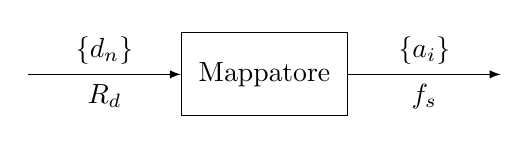
\begin{tikzpicture}[
                    node distance=3cm,
                    >=latex
                    ]
        
                    \node [coordinate] (input) {};
                    \node [draw, rectangle,right of = input, minimum height=3em, minimum width=6em] (block) {Mappatore};
                    \node [coordinate, right of = block] (output) {};
                    
                    \draw[draw,->] (input) --node[above]{$\{d_n$\}} node[below]{$R_d$} (block);
                    \draw[->] (block) --node[above]{$\{a_i$\}} node[below]{$f_s$} (output);
                \end{tikzpicture}    
            \end{figure}
            Ad esempio una mappa quaternaria:
            \begin{table}[H]
                \centering
                \begin{tabular}{c|c}
                $\{d_n\}$  & $\{a_i\}$ \\ \hline
                {00} & {-3}     \\
                {01} & {-1}     \\
                {10} & {1}     \\
                {11} & {3}    
                \end{tabular}
            \end{table}
            \begin{figure}[H]
                \centering
                \subfloat{
                    \begin{tikzpicture}
                        \begin{axis}[
                            xlabel=$t$,
                            ylabel=$d_n$,
                            xmin=-0.1,
                            xmax=5,
                            ymin=-0.2,
                            ymax=1,
                            ytick = {0,0.5},
                            xtick={0.5,1.5,2.5,3.5,4.5},
                            xticklabels={$1$,$0$,$1$,$1$},
                            % yticklabel style = {yshift=6pt,xshift=4pt}, 
                            yticklabels = {$0$,$1$},
                            axis lines=middle,
                            domain=-0.1:5,
                            samples=800,
                            width=6.5cm,
                            height=5cm
                        ]
                        \addplot [const plot, blue, thick] coordinates{(0,0.5)(1,0.5)(1,0)(2,0)(2,0.5)(4,0.5)(4,0)};
                        \addplot [const plot, dotted, blue] coordinates{(3,0)(3,0.5)};
                        \end{axis}
                    \end{tikzpicture}
                }
                \hfill
                \subfloat{
                    \begin{tikzpicture}
                        \begin{axis}[
                            xlabel=$t$,
                            ylabel=$a_i$,
                            xmin=-0.1,
                            xmax=5,
                            ymin=-1.5,
                            ymax=1.5,
                            ytick = {-1,-0.5,0.5,1},
                            yticklabels = {$-3$,$-1$,$1$,$3$,},
                            xtick={1,2},
                            xticklabels={$10$,$11$},
                            % yticklabel style = {yshift=6pt,xshift=4pt}, 
                            axis lines=middle,
                            domain=-0.1:5,
                            samples=800,
                            width=6.5cm,
                            height=6cm
                        ]
                        \addplot [const plot, blue, thick] coordinates{(0,0.5)(2,0.5)(2,1)(4,1)(4,-0.5)};
                    \end{axis}
                    \end{tikzpicture}
                }
            \end{figure}
            il periodo $T$ tra due \emph{simboli} adiacenti viene detto "Intervallo di Segnalazione". Se $M=2^q$ allora:
            \[
                T = qT_d =T_d log_{2}(M)  
            \]
            la velocitá di trasmissione dei simboli $f_s = \frac{1}{T}$ é legata al rate $R_d$ da:
            \[
                f_s = \frac{R_d}{Q} = \frac{R_d}{log_{2}(M)} 
            \] 
            devo caricare velocemente i simboli in ingresso al mappatore per poter completare la sequenza da mappare. Si nota anhe come
            all'aumentare della cardinalitá $M$ la velocitá diminuisca, la sua misura é fatta in $BAUD = \frac{simboli}{sec}$
        }
        \item {Mod: Modulatore converte la sequenza dei simboli $\{a_i\}$ in un segnale analogico $s_{T(t)}$ in modo tale da poter essere trasmesso  
            sul canale di comunicazione. Puó essere una modulazione {\color{blue}BB} o {\color{red}BP}, in ogni caso la banda impiegata sará:
            \[
                B_T \simeq \frac{1}{T}  
            \]
            volendolo esprimere in relazione ai vari bit rate:
            \[
                B_T = \frac{1}{T} \overset{T = qT_d}{=} \frac{1}{qT_d} = \frac{1}{T_d log_2(M)} = \frac{R_b}{\frac{n}{k} log_2(M)}     
            \]
            osserviamo come aumentando la cardinalitá $M$ della mappa riduco la banda, ció é molto utile per poter occupare uno spettro limitato ma ridurla troppo
            comporta un aumento dell'errore. Invece un rate del codice $\frac{n}{k}$ basso diminuisce le possibilitá di errore ma aumenta la banda occupata, si tendono 
            a usare codici che abbiano un rate vicino all'$1$. 
        }
    \end{itemize}
    Analizziamo la parte del ricevitore:
    \begin{figure}[H]
        \centering
            \begin{tikzpicture}[
                    node distance=3cm,
                    >=latex
                ]
                % Blocks
                \node [circle,draw] (RXant) {$r_{(t)}$};
                \node [rectangle, draw,minimum height=2em, minimum width=2em,right of=RXant] (RX) {$\substack{\text{Demodulatore}\\\text{Numerico}}$};
                \node [rectangle, draw,minimum height=2em, minimum width=2em,right of=RX] (DC) {Demappatore};
                \node [rectangle, draw,minimum height=2em, minimum width=2em,right of=DC] (DS) {$\substack{\text{Decodifica di}\\\text{canale}}$};
                \node [coordinate,right of = DS] (output) {};
            
                % Connections
                \draw [->] (RXant) --node[above]{} (RX);
                \draw [->] (RX) --node[above]{$\{\hat{a}_i\}$} (DC);
                \draw [->] (DC) --node[above]{$\{\hat{d}_n\}$} (DS);
                \draw [->] (DS) --node[above]{$\{\hat{b}_n\}$} (output);
            \end{tikzpicture}    
        \caption{Esempio sistema ricevitore}
    \end{figure}
    Il segnale ricevuto $r_{(t)}$ viene demodulato dal demodulatore numerico, il quale ha il compito di fornire una stima dei simboli $\{\hat{a}_i\}$ trasmessi.
    In seguito vengono demappati in modo da ottenere una stima di $\{\hat{d}_n\}$ dei bit di codice. Infine passano nel decodificatore di canale la quale uscita 
    fornisce ua stima dei $\{\hat{b}_n\}$ bit di informazione.

    I vantaggi di un sistema di comunicazione numerico rispetto ad uno analogico sono:
    \begin{itemize}
        \item {
            Una maggiore resistenza al rumore, dovuta all'alfabeto dei simboli limitato, che consente di prendere decisioni affidabili.
        }
        \item {
            La possibilitá di utilizzare ripetizioni rigenerative anziché ripetizioni che amplificano semplicemente il segnale ricevuto, amplificando quindi sia il segnale
            utile che il rumore. 
        }
        \item {
            La possibilitá di utilizzare codici a correzione d'errore inserendo ridondanza nella sequenza di bit informativi.
        }
    \end{itemize}
    \subsection{Phase Amplitude Modulation - PAM}
        É una tipologia di sistema di comunicazione in {\color{blue}Banda Base}, il cui segnale trasmesso $s_{T(t)}$ ha densitá spettrale
        di potenza centrata in $0$. Il sistema PAM riceve in ingresso simboli di modulazione $\{a_i\}$ provenienti dal mappaggio dei bit $\{d_n\}$ 
        \subsubsection{Mappatore}
            Il mappatore ha come cardinalitá una potenza del $2$, abbiamo PAM con mappatura: binaria, quaternaria o ottale
            \begin{table}[H]
                \centering
                \subfloat[Mappa Binaria]{
                    \begin{tabular}{c|c}
                        $\{d_n\}$  & $\{a_i\}$ \\ \hline
                        {0} & {-1}     \\
                        {1} & {+1}     \\
                    \end{tabular}
                }
                \hfill
                \subfloat[Mappa Quaternaria]{
                    \begin{tabular}{c|c}
                        $\{d_n\}$  & $\{a_i\}$ \\ \hline
                        {00} & {-3}     \\
                        {01} & {-1}     \\
                        {10} & {+1}     \\
                        {11} & {+3}    
                    \end{tabular}
                }
                \hfill
                \subfloat[Mappa Ottale]{
                    \begin{tabular}{c|c}
                        $\{d_n\}$  & $\{a_i\}$ \\ \hline
                        {000} & {-7}\\
                        {001} & {-5}\\
                        {010} & {-3}\\
                        {011} & {-1}\\
                        {100} & {+1}\\
                        {101} & {+3}\\
                        {110} & {+5}\\
                        {111} & {+7}    
                    \end{tabular}
                }
            \end{table}
            \begin{figure}[H]
                \centering
                    \begin{tikzpicture}[
                            node distance=3cm,
                            >=latex
                        ]
                        % Blocks
                        \node [coordinate,draw] (RX) {};
                        \node [rectangle, draw,minimum height=3em, minimum width=2em,right of=RX] (DC) {$\substack{\text{Mappatore}\\\text{PAM}}$};
                        \node [rectangle, draw,minimum height=3em, minimum width=2em,right of=DC] (DS) {$\substack{\text{Modulatore}\\\text{PAM}}$};
                        \node [coordinate,right of = DS] (output) {};
                    
                        % Connections
                        \draw [->] (RX) --node[above]{$\{d_n\}$}node[below]{$R_d$} (DC);
                        \draw [->] (DC) --node[above]{$\{a_i\}$}node[below]{$f_s$} (DS);
                        \draw [->] (DS) --node[above]{$s_{T(t)}$} (output);
                    \end{tikzpicture}    
                \caption{Sistema PAM}
            \end{figure}
        \subsubsection{Modulatore}
            Il segnale PAM é una serie di impulsi che si susseguono in successione con un intervallo $T = \frac{1}{f_s}$ e modulatori in ampiezza dei simboli 
            $\{a_i\}$. Possiamo usare un qualsiasi impulso, che chiamiamo $g_{T(t)}$, basta che sia di durata finita:
            \begin{figure}[H]
                \centering
                \subfloat{
                    \begin{tikzpicture}
                        \begin{axis}[
                            xlabel=$t$,
                            ylabel=$g_{T(t)}$,
                            xmin=-0.1,
                            xmax=3,
                            ymin=-0.2,
                            ymax=1.5,
                            ytick = {1},
                            yticklabels = {$1$},
                            xtick={1},
                            xticklabels={$T$},
                            % yticklabel style = {yshift=6pt,xshift=4pt}, 
                            axis lines=middle,
                            domain=-0.1:3,
                            samples=800,
                            width=6.5cm,
                            height=5cm
                        ]
                        \addplot [const plot, blue, thick] coordinates{(0,1)(1,1)(1,0)};
                        \end{axis}
                    \end{tikzpicture}
                }
                \hfill
                \subfloat{
                    \begin{tikzpicture}
                        \begin{axis}[
                            xlabel=$t$,
                            ylabel=$g_{T(t)}$,
                            xmin=-0.1,
                            xmax=3,
                            ymin=-0.2,
                            ymax=1.5,
                            ytick = {1},
                            yticklabels = {$1$},
                            xtick={1},
                            xticklabels={$T$},
                            % yticklabel style = {yshift=6pt,xshift=4pt}, 
                            axis lines=middle,
                            domain=-0.1:3,
                            samples=800,
                            width=6.5cm,
                            height=5cm
                        ]
                        \addplot [const plot, blue, thick, domain = 0:1] {gauss(0.5,0.3)-0.35};
                        % \addplot [const plot, blue, thick,domain=0:1,samples = 500] {gauss(0.5,1)};
                    \end{axis}
                    \end{tikzpicture}
                }
            \end{figure}
            se il segnale non fosse di durata finita $T$ avrei sovrapposizione dei segnali (un po come nella $TDF$ \ref{Teorema del Campionamento - Nyquist Shannon} se campiono male), il modulatore calcola ad ogni istante il segnale
            \[
                s_{T(t)} = \sum_{i}a_ig_{T(t-iT)}  
            \]
            nello schema a blocchi si riduce a
            \begin{figure}[H]
                \centering
                    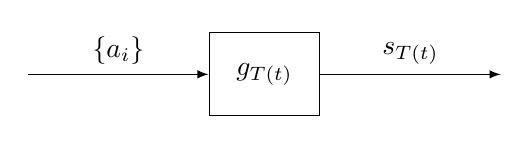
\begin{tikzpicture}[
                            node distance=3cm,
                            >=latex
                        ]
                        % Blocks
                        \node [coordinate,draw] (RX) {};
                        \node [rectangle, draw,minimum height=3em, minimum width=4em,right of=RX] (DC) {$g_{T(t)}$};
                        \node [coordinate,right of = DC] (output) {};
                    
                        % Connections
                        \draw [->] (RX) --node[above]{$\{a_i\}$} (DC);
                        \draw [->] (DC) --node[above]{$s_{T(t)}$} (output);
                    \end{tikzpicture}    
                \caption{Modulatore PAM}
            \end{figure}
            ne possiamo fare un esempio con una sequenza di simboli $\{a_i\} = \{+1,+3,-1,+1,-3\}$ e un impulso $g_{T(t)}$ del secondo tipo:
            \begin{figure}[H]
                \centering
                \subfloat[$\{a_i\}$]{
                    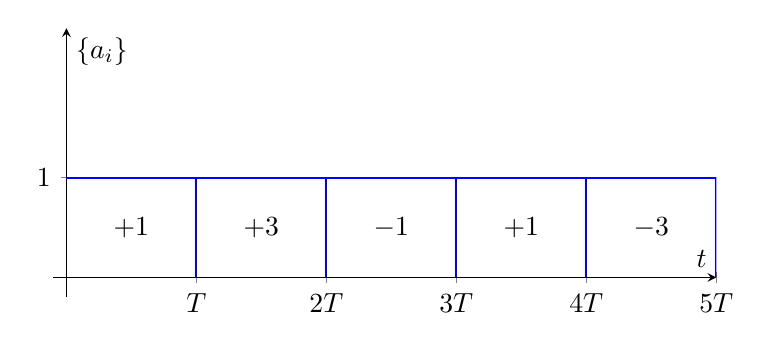
\begin{tikzpicture}
                        \begin{axis}[
                            xlabel=$t$,
                            ylabel=$\{a_i\}$,
                            xmin=-0.1,
                            xmax=5,
                            ymin=-0.2,
                            ymax=2.5,
                            ytick = {1},
                            yticklabels = {$1$},
                            xtick={1,2,3,4,5},
                            xticklabels={$T$,$2T$,$3T$,$4T$,$5T$},
                            % yticklabel style = {yshift=6pt,xshift=4pt}, 
                            axis lines=middle,
                            domain=-0.1:5,
                            samples=800,
                            width=10cm,
                            height=5cm
                        ]
                        \addplot [const plot, blue, thick] coordinates{(0,1)(1,1)(1,0)(1,1)(2,1)(2,0)(2,1)(3,1)(3,0)(3,1)(4,1)(4,0)(4,1)(5,1)(5,0)};
                        \node [] at (0.5,0.5) {$+1$};
                        \node [] at (1.5,0.5) {$+3$};
                        \node [] at (2.5,0.5) {$-1$};
                        \node [] at (3.5,0.5) {$+1$};
                        \node [] at (4.5,0.5) {$-3$};
                        \end{axis}
                    \end{tikzpicture}
                }
                \hfill
                \subfloat[$s_{T(t)}$]{
                    \begin{tikzpicture}
                        \begin{axis}[
                            xlabel=$t$,
                            ylabel=$s_{T(t)}$,
                            xmin=-0.1,
                            xmax=5,
                            ymin=-5,
                            ymax=5,
                            ytick = {1},
                            yticklabels = {$1$},
                            xtick={1,2,3,4,5},
                            xticklabels={$T$,$2T$,$3T$,$4T$,$5T$},
                            % yticklabel style = {yshift=6pt,xshift=4pt}, 
                            axis lines=middle,
                            domain=-0.1:5,
                            samples=800,
                            width=10cm,
                            height=8cm
                        ]
                        \addplot [const plot, orange, thick, domain = 0:1] {gauss(0.5,0.3)-0.34};
                        \addplot [const plot, orange, thick, domain = 1:2] {3*(gauss(1.5,0.3)-0.34)};
                        \addplot [const plot, orange, thick, domain = 2:3] {-gauss(2.5,0.3)+0.34};
                        \addplot [const plot, orange, thick, domain = 3:4] {gauss(3.5,0.3)-0.34};
                        \addplot [const plot, orange, thick, domain = 4:5] {-3*(gauss(4.5,0.3)-0.34)};
                        \addplot [const plot, dotted, thick] coordinates{(1,0)(1,5)};
                        \addplot [const plot, dotted, thick] coordinates{(2,0)(2,5)};
                        \addplot [const plot, dotted, thick] coordinates{(3,0)(3,5)};
                        \addplot [const plot, dotted, thick] coordinates{(4,0)(4,5)};
                        \addplot [const plot, dotted, thick] coordinates{(5,0)(5,5)};
                        \node [] at (0.5,3.5) {\small$a_0g_{T(t)}$};
                        \node [] at (1.5,3.5) {\small$a_1g_{T(t-T)}$};
                        \node [] at (2.5,3.5) {\small$a_2g_{T(t-2T)}$};
                        \node [] at (3.5,3.5) {\small$a_3g_{T(t-3T)}$};
                        \node [] at (4.5,3.5) {\small$a_4g_{T(t-4T)}$};

                        % \addplot [const plot, blue, thick,domain=0:1,samples = 500] {gauss(0.5,1)};
                    \end{axis}
                    \end{tikzpicture}
                }
            \end{figure}
            se invece utilizzassimo delle funzioni $g_{T(t)}$ rettangolari il segnale in uscita diventerebbe
            \begin{figure}[H]
                \centering
                \subfloat[$\{a_i\}$]{
                    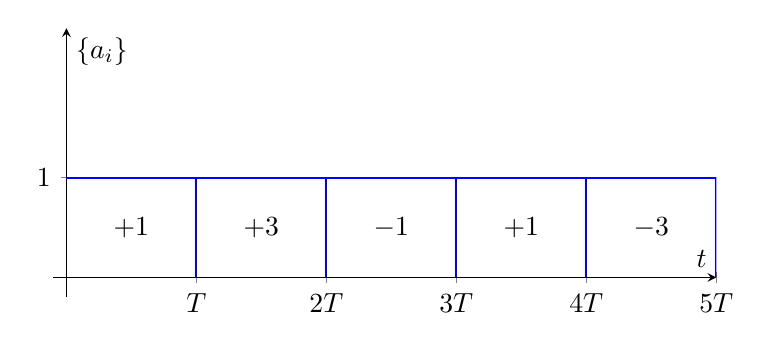
\begin{tikzpicture}
                        \begin{axis}[
                            xlabel=$t$,
                            ylabel=$\{a_i\}$,
                            xmin=-0.1,
                            xmax=5,
                            ymin=-0.2,
                            ymax=2.5,
                            ytick = {1},
                            yticklabels = {$1$},
                            xtick={1,2,3,4,5},
                            xticklabels={$T$,$2T$,$3T$,$4T$,$5T$},
                            % yticklabel style = {yshift=6pt,xshift=4pt}, 
                            axis lines=middle,
                            domain=-0.1:5,
                            samples=800,
                            width=10cm,
                            height=5cm
                        ]
                        \addplot [const plot, blue, thick] coordinates{(0,1)(1,1)(1,0)(1,1)(2,1)(2,0)(2,1)(3,1)(3,0)(3,1)(4,1)(4,0)(4,1)(5,1)(5,0)};
                        \node [] at (0.5,0.5) {$+1$};
                        \node [] at (1.5,0.5) {$+3$};
                        \node [] at (2.5,0.5) {$-1$};
                        \node [] at (3.5,0.5) {$+1$};
                        \node [] at (4.5,0.5) {$-3$};
                        \end{axis}
                    \end{tikzpicture}
                }
                \hfill
                \subfloat[$s_{T(t)}$]{
                    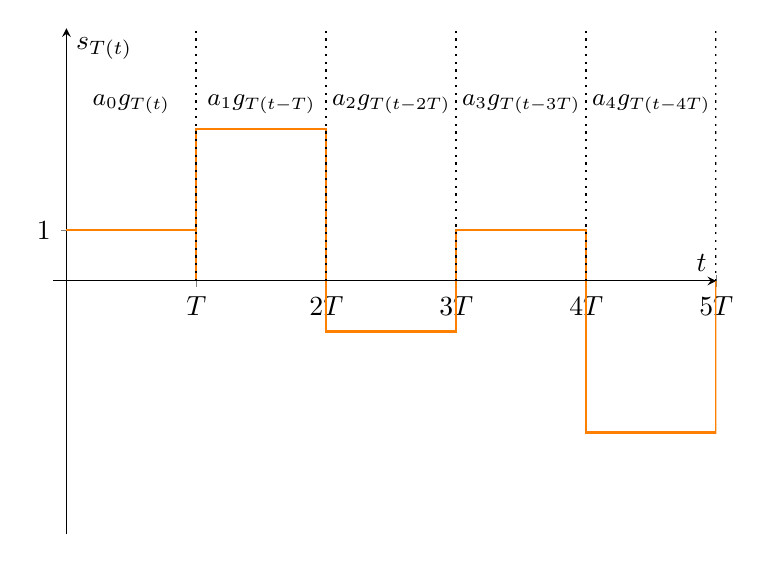
\begin{tikzpicture}
                        \begin{axis}[
                            xlabel=$t$,
                            ylabel=$s_{T(t)}$,
                            xmin=-0.1,
                            xmax=5,
                            ymin=-5,
                            ymax=5,
                            ytick = {1},
                            yticklabels = {$1$},
                            xtick={1,2,3,4,5},
                            xticklabels={$T$,$2T$,$3T$,$4T$,$5T$},
                            % yticklabel style = {yshift=6pt,xshift=4pt}, 
                            axis lines=middle,
                            domain=-0.1:5,
                            samples=800,
                            width=10cm,
                            height=8cm
                        ]
                        \addplot [const plot, orange, thick] coordinates{(0,1)(1,1)(1,0)(1,3)(2,3)(2,0)(2,-1)(3,-1)(3,0)(3,1)(4,1)(4,0)(4,-3)(5,-3)(5,0)};
                        \addplot [const plot, dotted, thick] coordinates{(1,0)(1,5)};
                        \addplot [const plot, dotted, thick] coordinates{(2,0)(2,5)};
                        \addplot [const plot, dotted, thick] coordinates{(3,0)(3,5)};
                        \addplot [const plot, dotted, thick] coordinates{(4,0)(4,5)};
                        \addplot [const plot, dotted, thick] coordinates{(5,0)(5,5)};
                        \node [] at (0.5,3.5) {\small$a_0g_{T(t)}$};
                        \node [] at (1.5,3.5) {\small$a_1g_{T(t-T)}$};
                        \node [] at (2.5,3.5) {\small$a_2g_{T(t-2T)}$};
                        \node [] at (3.5,3.5) {\small$a_3g_{T(t-3T)}$};
                        \node [] at (4.5,3.5) {\small$a_4g_{T(t-4T)}$};

                        % \addplot [const plot, blue, thick,domain=0:1,samples = 500] {gauss(0.5,1)};
                    \end{axis}
                    \end{tikzpicture}
                }
            \end{figure}
            dovendo analizzare il dominio frequnziale di $s_{T(t)}$ sarebbero tutte delle $sinc$ in {\color{blue}BB}  
        \subsubsection{Densitá spettrale di potenza}\label{Densita spettrale di potenza - PAM}
            Volendo analizzare la banda del segnale in uscita al modulatore PAM potremmo pensare di utilizzare la $TCF$:
            \begin{gather}
                s_{T(t)} \overset{TCF\ref{TCF di segnali periodici}}{\rightleftharpoons} S_{T(f)}\nonumber\\
                s_{T(t)}  = \sum_{i}a_i g_{T(t-iT)} \overset{TCF\ref{TCF di segnali periodici}}{\rightleftharpoons} \sum_{i}a_i G_{T(f)} e^{-j2\pi fiT}  \nonumber
            \end{gather}
            ma non posso analizzare con la $TCF$ le variabili aleatorie $a_i$. Posso allora calcolare la Densitá spettrale di potenza (\ref{Densita di potenza spettrale}).
            Ammettiamo che la sequenza di simboli di modulazione $\{a_i\}$ sia SSL \ref{Sitemi Stazionari in Senso Lato (SSL)}. La sua media é
            \[
                \mu_a = \eta_a = \mathbb{E}[a_i]
            \]  
            e la sua funzione di autocorrelazione
            \[
                R_{a(m)} = \mathbb{E}[a_ia_{i+m}]    
            \]
            ho la densitá spettrale di potenza come 
            \begin{gather}
                S_{s(f)} = \frac{1}{T} S_{a(f)}\left|G_{T(f)}\right|^2 \nonumber \\
                S_{a(f)} = \sum_{m} R_{a(m)}e^{-j2\pi fmT} \nonumber
            \end{gather}
            la cui formula finale ricorda quella di un processo SSL $S_{Y(f)} = S_{X(f)}\left|H_{(f)}\right|^2$, in questo
            caso dipende dalla $TCF$ del segnale $g_{T(t)}$ e dalla autocorrelazione dei simboli.
            \subsubsection{Potenza}
                Possiamo esprimere la potenza del segnale PAM come 
                \[
                    P_s =\int_{-\infty}^{\infty} S_{s(f)}df = \frac{1}{T}\int_{-\infty}^{\infty}S_{a(f)}  \left|G_{T(f)}\right|^2 df  \nonumber \\
                \]
                se i simboli $\{a_i\}$ sono incorrelati ho:
                \[
                    R_{a(m)} = 
                    \begin{cases}
                        \mathbb{E}\{a_i\} = \sigma_a^2 + \eta_a^2           & se\ m=0\nonumber\\    
                        \mathbb{E}\{a_i\}\mathbb{E}\{a_{i+m}\} = \eta_a^2   & se\ m\neq0\nonumber    
                    \end{cases}  
                \]
                semplificando la notazione della funzioe autocorrelazione diventa banalmente
                \[
                    R_{a(m)} =\eta_a^2 + \sigma_a^2\delta_{(m)} 
                \]
                \begin{figure}[H]
                    \centering
                    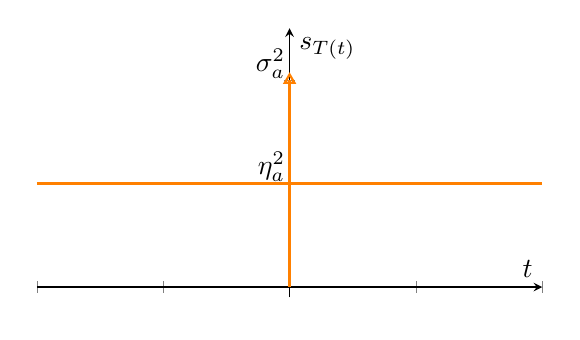
\begin{tikzpicture}
                        \begin{axis}[
                            xlabel=$t$,
                            ylabel=$s_{T(t)}$,
                            xmin=-4,
                            xmax=4,
                            ymin=-0.1,
                            ymax=2.5,
                            ytick = {1,2},
                            yticklabels = {$\eta_a^2$,$\sigma_a^2$},
                            xtick={},
                            xticklabels={},
                            yticklabel style = {yshift=6pt,xshift=4pt}, 
                            axis lines=middle,
                            domain=-4:4,
                            samples=800,
                            width=8cm,
                            height=5cm
                        ]
                        \addplot [const plot, orange, thick, samples = 500] {1};
                        \addplot+ [ycomb,mark = triangle, orange, thick, samples at = {0}] {2};
                    \end{axis}
                    \end{tikzpicture}
                \end{figure}
                dalla quale possiamo ricavare la densitá spettrale di potenza dei simboli
                \[
                    S_{a(f)} = \sigma_a^2 + \eta_a^2\sum_{m}e^{-j2\pi fmT} \overset{\ref{Relazione tra $TCF$ e $TDF$}}{=} \sigma_a^2 + \frac{\eta_a^2 }{T}\sum_{k} \delta_{(f-\frac{k}{T})}
                \]
                mentre la densitá spettrale di potenza del segnale 
                \begin{align}
                    S_{s(f)} &= \frac{1}{T} \left[\sigma_a^2 + \frac{\eta_a^2 }{T}\sum_{k} \delta_{(f-\frac{k}{T})}\right]\left|G_{T(f)}\right|^2 \nonumber \\
                            &= \frac{1}{T} \sigma_a^2\left|G_{T(f)}\right|^2 + \frac{\eta_a^2 }{T^2}\sum_{k} \delta_{(f-\frac{k}{T})}\left|G_{T(f)}\right|^2\nonumber \\
                            &\overset{\ref{Propietá del Delta di Dirac}}{=} \frac{1}{T} \sigma_a^2\left|G_{T(f)}\right|^2 + \frac{\eta_a^2 }{T^2}\sum_{k} \left|G_{T(\frac{k}{T})}\right|^2\nonumber
                \end{align}
                la potenza si calcola quindi con 
                \[
                    P_s  = \frac{\sigma_a^2}{T} E_{g_T} + \frac{\eta_a^2 }{T^2}\sum_{k} \left|G_{T(\frac{k}{T})}\right|^2
                \]
                dove $E_{g_T}$ per il Teorema di Parseval (\ref{Th. di Parseval}):
                \[
                    E_{g_T} = \int_{-\infty}^{\infty} \left|G_{T(f)}\right|^2 df 
                \]
                Possiamo osservare come una parte della potenza dipenda da una parte continua, $\frac{\sigma_a^2}{T} E_{g_T}$, e una parte discreta
                composta da un pettine di Delta di Dirac, $\frac{\eta_a^2 }{T^2}\sum_{k} \left|G_{T(\frac{k}{T})}\right|^2$. nel caso di simboli incorrelati ($\eta_a = 0$),
                e la parte continua dipende dal filtro con banda dimensionata rispetto a $\frac{1}{T}$, la banda del segnale trasmesso sará quindi $B_T \simeq \frac{1}{T}$. 
                La densitá spettrale di potenza in caso $\eta_a = 0$ diventa
                \[
                    S_{s(f)} = \frac{\sigma_a^2}{T} \left|G_{T(f)}\right|^2 =  \frac{\mathbb{E}[a_i^2]}{T} \left|G_{T(f)}\right|^2 = \frac{R_{a(0)}}{T} \left|G_{T(f)}\right|^2
                \] \label{Potenza - PAM}
                e di conseguenza la potenza 
                \[
                    P_s  = \frac{\sigma_a^2}{T} E_{g_T} = \frac{\mathbb{E}[a_i^2]}{T} E_{g_T} = \frac{R_{a(0)}}{T} E_{g_T}
                \]
        \subsubsection{Potenza e Energia - caso IID}
            Consideriamo adesso un sistema PAM con simboli indipendenti ed identicamente distribuiti (IID)
            \[
                \eta_a = 0 \hspace{1cm} \sigma_a^2 = \mathbb{E}[a_i^2] = \frac{M^2-1}{3}    
            \]
            con $M$ la cardinalitá del mappatore, risultano 
            \begin{itemize}
                \item {Densitá spettrale di potenza:
                    \[
                        S_{s(f)} = \frac{M^2-1}{3T}\left|G_{T(f)}\right|^2
                    \]
                }
                \item {Potenza:
                    \[
                        P_s = \frac{M^2-1}{3T}E_{g_T}
                    \]
                }
                \item {Energia media per simbolo: dato che l'energia é calcolata in un $\Delta t$ posso ricavare l'energia del simbolo moltiplicando la potenza per $T$
                    \[
                        E_S = P_sT = \frac{M^2-1}{3}E_{g_T}
                    \]
                }
                \item {Energia media per bit: dato che l'energia é calcolata in un $\Delta t$ posso ricavare l'energia del bit da trasmettere
                moltiplicando la potenza per $T_d$
                    \[
                        E_d = P_sT_d = \frac{M^2-1}{3log_2(M)}E_{g_T}
                    \]
                }
            \end{itemize}
        \subsubsection{Schema completo di un sistema di comunicazione PAM}
            \begin{figure}[H]
                \centering
                    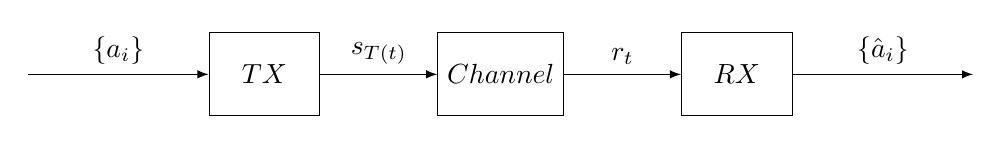
\begin{tikzpicture}[
                            node distance=3cm,
                            >=latex
                        ]
                        % Blocks
                        \node [coordinate,draw] (in) {};
                        \node [rectangle, draw,minimum height=3em, minimum width=4em,right of=in] (TX) {$TX$};
                        \node [rectangle, draw,minimum height=3em, minimum width=4em,right of=TX] (C) {$Channel$};
                        \node [rectangle, draw,minimum height=3em, minimum width=4em,right of=C] (RX) {$RX$};
                        \node [coordinate,right of = RX] (output) {};
                    
                        % Connections
                        \draw [->] (in) --node[above]{$\{a_i\}$} (TX);
                        \draw [->] (TX) --node[above]{$s_{T(t)}$} (C);
                        \draw [->] (C) --node[above]{$r_{t}$} (RX);
                        \draw [->] (RX) --node[above]{$\{\hat{a}_i\}$} (output);
                    \end{tikzpicture}    
                \caption{Sistema PAM generico}
            \end{figure}
            i singoli componenti racchiudono

            \begin{figure}[H]
                \centering
                \subfloat[TX]{
                    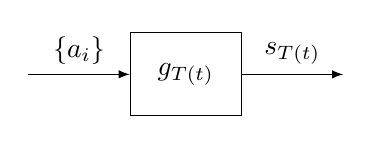
\begin{tikzpicture}[
                            node distance=2cm,
                            >=latex
                        ]
                        % Blocks
                        \node [coordinate,draw] (in) {};
                        \node [rectangle, draw,minimum height=3em, minimum width=4em,right of=in] (TX) {$g_{T(t)}$};
                        \node [coordinate,right of = TX] (output) {};
                    
                        % Connections
                        \draw [->] (in) --node[above]{$\{a_i\}$} (TX);
                        \draw [->] (TX) --node[above]{$s_{T(t)}$} (output);
                    \end{tikzpicture}    
                }
                \hfill
                \subfloat[Channel]{
                    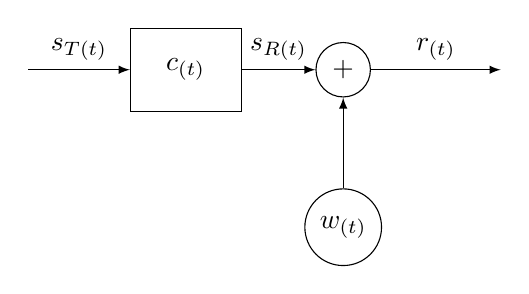
\begin{tikzpicture}[
                            node distance=2cm,
                            >=latex
                        ]
                        % Blocks
                        \node [coordinate,draw] (in) {};
                        \node [rectangle, draw,minimum height=3em, minimum width=4em,right of=in] (TX) {$c_{(t)}$};
                        \node [circle, draw,right of=TX] (C) {$+$};
                        \node [circle,draw,below of=C] (error) {$w_{(t)}$};
                        \node [coordinate,right of = C] (output) {};
                    
                        % Connections
                        \draw [->] (in) --node[above]{$s_{T(t)}$} (TX);
                        \draw [->] (TX) --node[above]{$s_{R(t)}$} (C);
                        \draw [->] (error) -- (C);
                        \draw [->] (C) --node[above]{$r_{(t)}$} (output);
                    \end{tikzpicture}    
                }
                \hfill
                \subfloat[RX]{
                    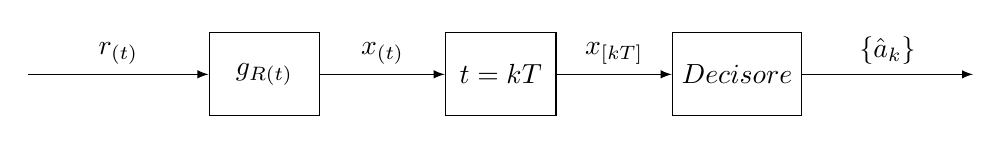
\begin{tikzpicture}[
                            node distance=3cm,
                            >=latex
                        ]
                        % Blocks
                        \node [coordinate,draw] (in) {};
                        \node [rectangle, draw,minimum height=3em, minimum width=4em,right of=in] (TX) {$g_{R(t)}$};
                        \node [rectangle, draw,minimum height=3em, minimum width=4em,right of=TX] (C) {$t=kT$};
                        \node [rectangle, draw,minimum height=3em, minimum width=4em,right of=C] (RX) {$Decisore$};
                        \node [coordinate,right of = RX] (output) {};
                    
                        % Connections
                        \draw [->] (in) --node[above]{$r_{(t)}$} (TX);
                        \draw [->] (TX) --node[above]{$x_{(t)}$} (C);
                        \draw [->] (C) --node[above]{$x_{[kT]}$} (RX);
                        \draw [->] (RX) --node[above]{$\{\hat{a}_k\}$} (output);
                    \end{tikzpicture}    
                }
            \end{figure}
            \begin{itemize}
                \item {$\{a_i\}$: sequenza di simboli di modulazione, generati con frequenza $f_s=\frac{1}{T}$ e appartenenti all'alfabeto
                \[
                    A = \{\pm 1,\pm 3, \dots, \pm (M-1),\}  
                \]}
                \item {$g_{T(t)}$: impulso di trasmissione}
                \item {$c_{(t)}$: risposta impulsiva del canale}
                \item {$w_{(t)}$: rimore gaussiano bianco con densitá spettrale di potenza\[
                    S_{w(f)} = \frac{N_0}{2}  
                \]}
                \item {$g_{T(t)}$: filtro di ricezione}
                \item {$\{\hat{a}_k\}$: stima dei simboli}
            \end{itemize}
            Analizziamo come varia il segnale al passaggio dei vari stadi:
            \begin{itemize}
                \item {Segnale trasmesso:
                    \[
                        s_{T(t)} = \sum_{i}a_ig_{T(t-iT)}  
                    \]
                }
                \item {Segnale utile ricevuto:
                    \[
                        s_{R(t)} = s_{T(t)} \otimes c_{(t)} = \sum_{i}a_ig_{TC(t-iT)}  
                    \]
                    con 
                    \[
                        g_{TC(t)} = g_{T(t)} \otimes c_{(t)} 
                    \]
                }
                \item {Segnale ricevuto:
                    \[
                        r_{(t)} = s_{R(t)} + w_{(t)}  
                    \]
                }
                \item {Segnale in uscita dal filtro di ricezione:
                    \[
                        x_{(t)} = r_{(t)} \otimes g_{R(t)} = \sum_{i}a_ig_{(t-iT)}+n_{(t)}  
                    \]
                    dove $g_{(t)}$ é la risposta impulsiva globale del sistema
                    \[
                        g_{(t)} = g_{TC(t)} \otimes g_{R(t)} = g_{T(t)} \otimes c_{(t)} \otimes g_{R(t)}
                    \]
                    e la componente del rumore 
                    \[
                        n_{(t)} = w_{(t)} \otimes g_{R(t)}    
                    \]
                    esso é un processo Gaussiano a media nulla e densitá spettrale di potenza 
                    \[
                        S_{n(f)} = \frac{N_0}{2} \left|G_{R(f)}\right|^2  
                    \]
                }
                \item {Componente ricevuta:
                    \[
                        x_{[kT]} = \sum_{i}a_ig_{[(n-i)T]}+n_{[k]}  
                    \]
                    dove $n_{[k]}$ é una variabile aleatoria Gaussiana a media nulla e varianza 
                    \[
                        \sigma_n^2 = \frac{N_0}{2} \int_{-\infty}^{\infty}\left|G_{R(f)}\right|^2 df =\frac{N_0}{2} E_{g_R} 
                    \]
                    essendo $E_{g_R}$ l'energia di $g_{R(t)}$, con il cambio d'indice $k-i = m$ il campione in uscita dal filtro di ricezione
                    assume la forma 
                    \[
                        x_{[kT]} = \sum_{m}a_{k-m}g_{[mT]}+n_{[k]}
                    \]
                    isolando il termine relativo $m=0$
                    \[
                        x_{[kT]} = a_Kg_{(0)} + \sum_{m\neq 0}a_{k-m}g_{[mT]}+n_{[k]}      
                    \]
                    Il campione $x_{[kT]}$ viene utilizzato per prendere una decisione sul simbolo $a_k$ il termine utile nella espressione di $x_{[kT]}$
                    é 
                    \[
                        a_Kg_{(0)}
                    \]\label{ISI}
                    il secondo termine che appare é il cntributo di tutti i simboli di modulazione diversi da $a_k$ e rappresenta un disturbo che si 
                    sovrappone al termine utile. Il disturbo descritto prende il nome di \emph{Interferenza Intersimbolica} (ISI)
                    \[
                        ISI =  \sum_{m\neq 0}a_{k-m}g_{[mT]}
                    \]
                    Notiamo come noi possiamo operare su:
                    \begin{itemize}
                        \item {
                            $g_T$ e $g_R$ per agire in modo congiunto sull'interferenza intersimbolica con l'obbiettivo di renderla nulla
                        }
                        \item {
                            $g_R$ agisce sul rumore termico $S_{n(f)} = \frac{N_0}{2} \left|G_{R(f)}\right|^2$
                        }
                    \end{itemize}
                    Infine $n_k$ é il contributo del rumore termico. Rispetto ai sistemi di comunicazione analogici nei sistemi di comunicazione numerici
                    é presente un'altra forma di disturbo l'ISI, normalmente l'ISI ha ordini di grandezza molto superiori al rumore termico per cui bisogna 
                    eliminarlo.
                }
            \end{itemize}
        \subsubsection{Rimozione dell'ISI}
            Riprendendo l'equazione dell'ISI
            \[
                ISI =  \sum_{m\neq 0}a_{k-m}g_{[mT]}
            \]
            si nota come il suo completo annullamento é possibile imponendo le condizioni di Nyquist \label{Condizioni di Nyquist} nel dominio del tempo
            \[
                g_{[mT]} = 
                \begin{cases}
                    1   &per \ m=0\nonumber \\
                    0   &per \ m\neq 0\nonumber
                \end{cases}  
            \]
            ricordiamo che $g_{(t)} = g_{T(t)} \otimes c_{(t)} \otimes g_{R(t)}$, allora l'espressione delle componenti 
            ricevute diventa
            \[
                x_{[kT]} = a_k+n_{[k]}  
            \]
            costituita dal simbolo trasmesso $a_k$ e dal rumore $n_k$. Un impulso che soddisfa tali condizioni si dice \emph{Impulso di Nyquist}.
            Sono quindi condizioni sufficienti, per $g_(t)$, che sia nullo agli estremi dell'intervallo $[-kT,kT]$ e che sia non nulla in $t=0$
            allora soddisfano le codizioni di Nyquist
            \begin{figure}[H]
                \centering
                    \begin{tikzpicture}
                        \begin{axis}[
                            xlabel=$t$,
                            ylabel=$g_{(t)}$,
                            xmin=-4,
                            xmax=4,
                            ymin=-0.1,
                            ymax=2.5,
                            ytick = {},
                            yticklabels = {},
                            xtick={-4,-3,-2,-1,1,2,3,4},
                            xticklabels={$-4T$,$-3T$,$-2T$,$-T$,$T$,$2T$,$3T$,$4T$},
                            axis lines=middle,
                            domain=-4:4,
                            samples=800,
                            width=9cm,
                            height=6cm
                        ]
                        \addplot+ [ycomb,red, thick, samples at = {-4,-3,-2,-1,0,1,2,3,4}] {gauss(0,0.3)};
                        \addplot [const plot, blue, thick, samples = 500] {gauss(0,0.3)};
                    \end{axis}
                    \end{tikzpicture}                
            \end{figure}
            ma le condizioni ci dicono che anche un segnale che si annulla a intervalli di $kT$ soddisfa le condizioni
            \begin{figure}[H]
                \centering
                    \begin{tikzpicture}
                        \begin{axis}[
                            xlabel=$t$,
                            ylabel=$g_{(t)}$,
                            xmin=-4,
                            xmax=4,
                            ymin=-2,
                            ymax=2,
                            ytick = {},
                            yticklabels = {},
                            xtick={-4,-3,-2,-1,1,2,3,4},
                            xticklabels={$-4T$,$-3T$,$-2T$,$-T$,$T$,$2T$,$3T$,$4T$},
                            axis lines=middle,
                            domain=-4:4,
                            samples=800,
                            width=9cm,
                            height=6cm
                        ]
                        \addplot [blue, thick, samples = 100] {sin(deg(x*pi))/(x*pi)};
                        \addplot+ [ycomb, blue, thick, samples at = {-4,-3,-2,-1,0,1,2,3,4}] {gauss(0,0.4)};
                    \end{axis}
                    \end{tikzpicture}                
            \end{figure}
            ad esempio prendiamo $g_R=g_T=rect\left(\frac{t}{T}\right)$ e il canale $c_{(t)} = \delta_{(t)}$
            \begin{figure}[H]
                \centering
                    \begin{tikzpicture}
                        \begin{axis}[
                            xlabel=$t$,
                            ylabel=$g_{(t)}$,
                            xmin=-4,
                            xmax=4,
                            ymin=-0.1,
                            ymax=2.5,
                            ytick = {},
                            yticklabels = {},
                            xtick={-1,1},
                            xticklabels={$-\frac{T}{2}$,$\frac{T}{2}$},
                            axis lines=middle,
                            domain=-4:4,
                            samples=800,
                            width=9cm,
                            height=6cm
                        ]
                        \addplot [const plot, blue, thick] coordinates{(-1,0)(-1,1)(1,1)(1,0)};
                        \addplot+ [ycomb, purple,mark = triangle, thick, samples at = {0}] {1.5};
                    \end{axis}
                    \end{tikzpicture}      
                    \caption{{\color{blue}$g_R=g_T$},{\color{purple}$c_{(t)}$}}          
            \end{figure}
            se ne calcolo il prodotto di convoluzione
            \begin{figure}[H]
                \centering
                    \begin{tikzpicture}
                        \begin{axis}[
                            xlabel=$t$,
                            ylabel=$g_{(t)}$,
                            xmin=-4,
                            xmax=4,
                            ymin=-0.1,
                            ymax=2.5,
                            ytick = {},
                            yticklabels = {},
                            xtick={-2,2},
                            xticklabels={$-T$,$T$},
                            axis lines=middle,
                            domain=-4:4,
                            samples=800,
                            width=9cm,
                            height=6cm
                        ]
                        \addplot [sharp plot, blue, thick] coordinates{(-2,0)(0,1)(2,0)};
                    \end{axis}
                    \end{tikzpicture}      
                    \caption{$g_{(t)}$}          
            \end{figure}
            la quale $g_{(t)}$ soddisfa le condizioni di Nyquist.
            \paragraph{Condizioni di Nyquist - Dominio della frequenza} Traduciamo le condizioni di Nyquist nel dominio della frequenza. Partendo
            dalla trasformata di Fourier di $g_{(t)}$
            \[
                G_{(f)} =\int_{-\infty}^{\infty}g_{(t)}e^{-j2\pi ft}    
            \]
            e la trasformata di $g_{[mT]}$
            \[
                \overline{G_{(f)}} \overset{\ref{TDF}}{\rightleftharpoons}\sum_{m}g_{[mT]}e^{-j2\pi fmT}    
            \]
            per le relazioni tra $TCF$ e $TDF$ (\ref{Relazione tra $TCF$ e $TDF$})
            \[
                \overline{G_{(f)}} \overset{\ref{TDF}}{\rightleftharpoons}\frac{1}{T}\sum_{k}G_{(f-\frac{k}{T})}    
            \]
            se sono valide le condizioni di Nyquist
            \[
                \begin{cases}
                    g_{(0)} & m=0\nonumber \\
                    0 &\nonumber
                \end{cases}  \Rightarrow \overline{G_{(f)}} = g_{(0)} 
            \]
            ho solo il termine per $m=0$ e di conseguenza ho ISI nullo. Questo vuol dire che finché la somma delle ripetizioni
            della $G_{(f)}$ a intervalli di $\frac{1}{T}$ é uguale a una costante su tutto l'asse delel frequenze l'ISI é nullo.
            Un esempio con $G_{(f)} = triangoli,\ g_{(t)} = sinc^2$ con turata $\frac{1}{2T}$
            \begin{figure}[H]
                \centering
                    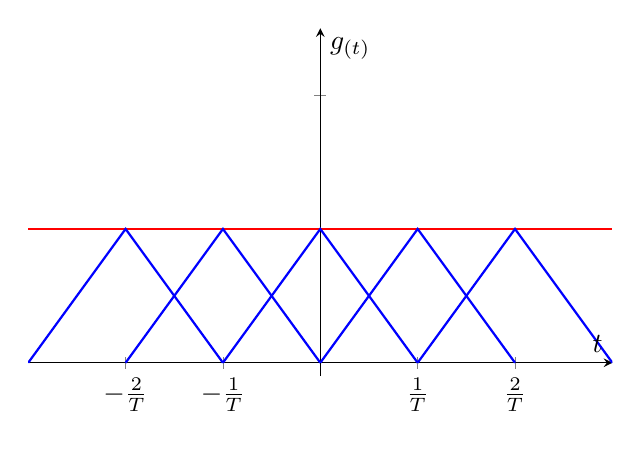
\begin{tikzpicture}
                        \begin{axis}[
                            xlabel=$t$,
                            ylabel=$g_{(t)}$,
                            xmin=-6,
                            xmax=6,
                            ymin=-0.1,
                            ymax=2.5,
                            ytick = {},
                            yticklabels = {},
                            xtick={-4,-2,2,4},
                            xticklabels={$-\frac{2}{T}$,$-\frac{1}{T}$,$\frac{1}{T}$,$\frac{2}{T}$},
                            axis lines=middle,
                            domain=-6:6,
                            samples=800,
                            width=9cm,
                            height=6cm
                        ]
                        \addplot [sharp plot, red, thick] coordinates{(-6,1)(6,1)};
                        \addplot [sharp plot, blue, thick] coordinates{(-2,0)(0,1)(2,0)};
                        \addplot [sharp plot, blue, thick] coordinates{(-4,0)(-2,1)(0,0)};
                        \addplot [sharp plot, blue, thick] coordinates{(-6,0)(-4,1)(-2,0)};
                        \addplot [sharp plot, blue, thick] coordinates{(4,0)(2,1)(0,0)};
                        \addplot [sharp plot, blue, thick] coordinates{(6,0)(4,1)(2,0)};
                    \end{axis}
                    \end{tikzpicture}      
                    \caption{$g_{(t)}$}          
            \end{figure}
            ma non tutte le tipologie di triangoli ad esempio vanno bene, ad esempio se la durata fosse inferiore
            \begin{figure}[H]
                \centering
                    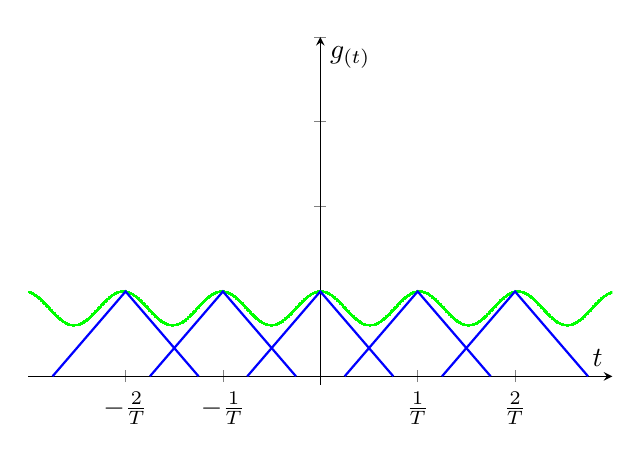
\begin{tikzpicture}
                        \begin{axis}[
                            xlabel=$t$,
                            ylabel=$g_{(t)}$,
                            xmin=-6,
                            xmax=6,
                            ymin=-0.1,
                            ymax=4,
                            ytick = {},
                            yticklabels = {},
                            xtick={-4,-2,2,4},
                            xticklabels={$-\frac{2}{T}$,$-\frac{1}{T}$,$\frac{1}{T}$,$\frac{2}{T}$},
                            axis lines=middle,
                            domain=-6:6,
                            samples=800,
                            width=9cm,
                            height=6cm
                        ]
                        \addplot [const plot, thick, green, samples = 800] {0.2*cos(deg(3.1*x))+0.8};
                        \addplot [sharp plot, blue, thick] coordinates{(-1.5,0)(0,1)(1.5,0)};
                        \addplot [sharp plot, blue, thick] coordinates{(-3.5,0)(-2,1)(-0.5,0)};
                        \addplot [sharp plot, blue, thick] coordinates{(-5.5,0)(-4,1)(-2.5,0)};
                        
                        \addplot [sharp plot, blue, thick] coordinates{(3.5,0)(2,1)(0.5,0)};
                        \addplot [sharp plot, blue, thick] coordinates{(5.5,0)(4,1)(2.5,0)};
                    \end{axis}
                    \end{tikzpicture}      
                    \caption{$g_{(t)}$}          
            \end{figure}
            \paragraph*{Banda Minima di Nyquist:} Le condizioni di Nyquist nel dominio della frequenza
            \[
                \sum_{k= -\infty}^{\infty} G_{(f-\frac{k}{T})} = T
            \]
            indicano che una condizione \emph{necessaria}, ma non sufficiente, affinché un impulso $g_{(t)}$ sia di Nyquist
            é che la sua trasformata di Fourier $G_{(f)}$ abbia banda almeno pari a $\frac{1}{2T}$. Se cosí non fosse
            le ripetizioni della trasformata $G_{(f)}$ nel dominio della frequenza sarebbe nulla in $f=\frac{1}{2T}$ e non sarebbero
            piú soddisfatte le condizioni di Nyquist nel dominio della frequenza come ad esempio
            \begin{figure}[H]
                \centering
                    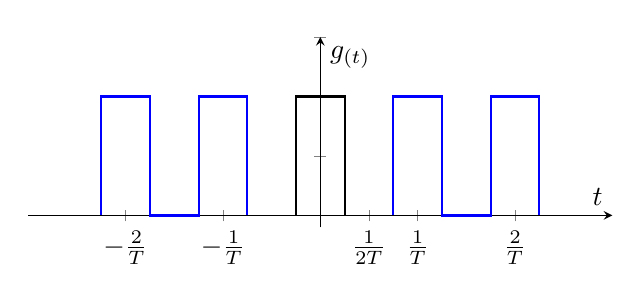
\begin{tikzpicture}
                        \begin{axis}[
                            xlabel=$t$,
                            ylabel=$g_{(t)}$,
                            xmin=-6,
                            xmax=6,
                            ymin=-0.1,
                            ymax=1.5,
                            ytick = {},
                            yticklabels = {},
                            xtick={-4,-2,1,2,4},
                            xticklabels={$-\frac{2}{T}$,$-\frac{1}{T}$,$\frac{1}{2T}$,$\frac{1}{T}$,$\frac{2}{T}$},
                            axis lines=middle,
                            domain=-6:6,
                            samples=800,
                            width=9cm,
                            height=4cm
                        ]
                        \addplot [const plot, black, thick] coordinates{(-0.5,0)(-0.5,1)(0.5,1)(0.5,0)};
                        \addplot [const plot, blue, thick] coordinates{(1.5,0)(1.5,1)(2.5,1)(2.5,0)(3.5,0)(3.5,1)(4.5,1)(4.5,0)};
                        \addplot [const plot, blue, thick] coordinates{(-1.5,0)(-1.5,1)(-2.5,1)(-2.5,0)(-3.5,0)(-3.5,1)(-4.5,1)(-4.5,0)};
                    \end{axis}
                    \end{tikzpicture}      
                    \caption{$g_{(t)}$}          
            \end{figure}
            la banda $B_N =\frac{1}{2T}$ é detta banda minima di Nyquist, é un condizione necessara ma non sufficiente, per l'eliminazione di ISI,
            poiché se gli impulsi sono di banda maggiore a $B_N$ la somma delle ripetizioni di $G_{(f)}$ non é una costante
            \begin{figure}[H]
                \centering
                \subfloat[$g_{(t)}$]{
                    \begin{tikzpicture}
                        \begin{axis}[
                            xlabel=$t$,
                            ylabel=$g_{(t)}$,
                            xmin=-4,
                            xmax=4,
                            ymin=-0.1,
                            ymax=2,
                            ytick = {},
                            yticklabels = {},
                            xtick={-4,-2,-1,1,2,4},
                            xticklabels={$-\frac{2}{T}$,$-\frac{1}{T}$,$-\frac{1}{2T}$,$\frac{1}{2T}$,$\frac{1}{T}$,$\frac{2}{T}$},
                            axis lines=middle,
                            domain=-4:4,
                            samples=800,
                            width=10cm,
                            height=4cm
                        ]
                        \addplot [const plot, blue, thick] coordinates{(-1.5,0)(-1.5,1)(1.5,1)(1.5,0)};
                    \end{axis}
                    \end{tikzpicture}
                }
                \hfill
                \subfloat[{\color{green}$\sum G_{(f-\frac{k}{T})}$}]{
                    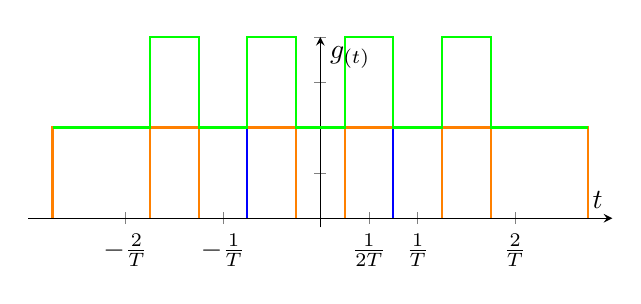
\begin{tikzpicture}
                        \begin{axis}[
                            xlabel=$t$,
                            ylabel=$g_{(t)}$,
                            xmin=-6,
                            xmax=6,
                            ymin=-0.1,
                            ymax=2,
                            ytick = {},
                            yticklabels = {},
                            xtick={-4,-2,1,2,4},
                            xticklabels={$-\frac{2}{T}$,$-\frac{1}{T}$,$\frac{1}{2T}$,$\frac{1}{T}$,$\frac{2}{T}$},
                            axis lines=middle,
                            domain=-6:6,
                            samples=800,
                            width=9cm,
                            height=4cm
                        ]
                        \addplot [const plot, blue, thick] coordinates{(-1.5,0)(-1.5,1)(1.5,1)(1.5,0)};
                        \addplot [const plot, orange, thick] coordinates{(0.5,0)(0.5,1)(3.5,1)(3.5,0)};
                        \addplot [const plot, orange, thick] coordinates{(2.5,0)(2.5,1)(5.5,1)(5.5,0)};

                        \addplot [const plot, orange, thick] coordinates{(-0.5,0)(-0.5,1)(-3.5,1)(-3.5,0)};
                        \addplot [const plot, orange, thick] coordinates{(-2.5,0)(-2.5,1)(-5.5,1)(-5.5,0)};

                        \addplot [const plot, green, thick] coordinates{(-5.5,1)(-3.5,1)(-3.5,2)(-2.5,2)(-2.5,1)(-1.5,1)(-1.5,2)(-0.5,2)(-0.5,1)(0.5,1)(0.5,2)(1.5,2)(1.5,1)(2.5,1)(2.5,2)(3.5,2)(3.5,1)(5.5,1)};
                    \end{axis}
                    \end{tikzpicture}
                }      
            \end{figure}
            l'impulso quindi deve avere banda minima di Nyquist di solito viene identificato da una funzione con trasformata di Fourier 
            rettangolare 
            \[
                G_{(f)} = g_{(0)} rect(fT)  
            \]
            e nel tempo
            \[
                g_{(t)} = g_{(0)}\frac{1}{T}sinc\left(\frac{t}{T}\right)
            \]
            \begin{figure}[H]
                \centering
                \subfloat[$G_{(f)}$]{
                        \begin{tikzpicture}
                        \begin{axis}[
                            xlabel=$f$,
                            ylabel=$G_{(f)}$,
                            xmin=-4,
                            xmax=4,
                            ymin=-0.1,
                            ymax=2,
                            ytick = {},
                            yticklabels = {},
                            xtick={-2,2},
                            xticklabels={$-\frac{1}{2T}$,$\frac{1}{2T}$},
                            axis lines=middle,
                            domain=-4:4,
                            samples=800,
                            width=6.5cm,
                            height=4cm
                        ]
                        \addplot [const plot, blue, thick] coordinates{(-2,0)(-2,1)(2,1)(2,0)};
                    \end{axis}
                    \end{tikzpicture}
                }
                \hfill
                \subfloat[$g_{(t)}$]{
                    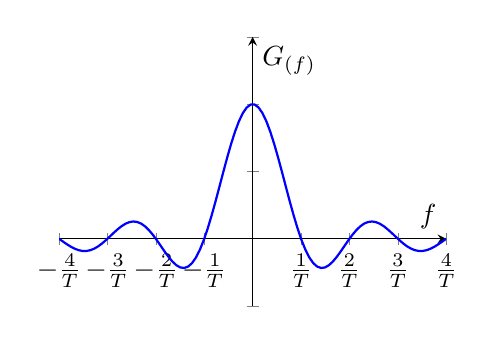
\begin{tikzpicture}
                        \begin{axis}[
                            xlabel=$f$,
                            ylabel=$G_{(f)}$,
                            xmin=-4,
                            xmax=4,
                            ymin=-0.5,
                            ymax=1.5,
                            ytick = {},
                            yticklabels = {},
                            xtick={-4,-3,-2,-1,1,2,3,4},
                            xticklabels={$-\frac{4}{T}$,$-\frac{3}{T}$,$-\frac{2}{T}$,$-\frac{1}{T}$,$\frac{1}{T}$,$\frac{2}{T}$,$\frac{3}{T}$,$\frac{4}{T}$},
                            axis lines=middle,
                            domain=-4:4,
                            samples=800,
                            width=6.5cm,
                            height=5cm
                        ]
                        \addplot [blue, thick, samples = 100] {sin(deg(x*pi))/(x*pi)};
                    \end{axis}
                    \end{tikzpicture}
                }
                
            \end{figure}
        \paragraph{Dimensionaento di $g_{(t)}$}
            Riprendiamo il segnale in ricezione di un sistema PAM
            \[
                x_{[k]} = \sum_{m} a_{k-m}g_{[mT]} + n_{[k]}   
            \]
            con 
            \begin{gather}
                g_{(t)} = g_{T(t)} \otimes c_{(t)} \otimes g_{R(t)}\nonumber \\
                n_{[k]} = n_{(t=mT)}:\ S_{n(f)} = \frac{N_0}{2} \left|G_{R(f)}\right|^2\nonumber
            \end{gather}
            il decisore si basa sulla variabile $a_k$
            \[
                x_{[k]} = a_{k}g_{(0)} + \sum_{m\neq 0} a_{k-m}g_{[mT]}    
            \]
            dove:
            \begin{itemize}
                \item {$a_{k}g_{(0)}$ é la componente utile}
                \item {$\sum_{m\neq 0} a_{k-m}g_{[mT]}$ é l'ISI, il quale si annulla per le condizioni di Nyquist:
                        \begin{itemize}
                            \item {Nel tempo:
                                \[
                                    g_{(mT)} = 
                                    \begin{cases}
                                        g_{(0)} &m=0\nonumber \\
                                        0 &m\neq 0\nonumber 
                                    \end{cases}  
                                \]
                            }
                            \item {Nella Frequenza: faccio la $TDF$ delle condizioni nel tempo
                                \[
                                    \overline{G_{(f)}} = g_{(0)} = \sum_{k}\frac{1}{T}G_{(f-\frac{k}{T})}    
                                \]
                                la quale é vera se la banda minima, $B_{min}$, di $G_{(f)}$ é $\frac{1}{2T}$. La 
                                funzione che soddisfa tali condizioni é una $rect$ che nel dominio del tempo é una $sinc$
                            }
                        \end{itemize}
                }
            \end{itemize}
            in realtá non uso la $rect/sinc$ per realizzare il dimensionaemnto della $g_{(t)}$ 
            \begin{itemize}
                \item {In frequenza la $rect$ é discontinua, é difficile realizzare le 2 spike a $\pm\frac{1}{2T}$}
                \item {Nel dominio del tempo ho una $sinc$ che é infinita, ed un eventuale errore di sincronizzazione
                (\ref{Errore Sincronizzazione}) introduce ISI}
            \end{itemize}
            Le ipotesi che abbiamo fatto fino ad ora implicano che il riceviore riesca a campionare a istanti
            di tempo $T$, ma il $T$ é un parametro che sceglie il trasmettitore, di conseguenza \label{Errore Sincronizzazione}
            i due dispositivi si devono sincronizzare e decidere un $T$. Il ricevitore comunque non riesce a campionare
            precisamente a $T$, per motivi di trasmissione o non si sincronizza perfettamente, avró un leggero delta di campionamento
            \[
                T_c = T+ \tau  
            \]
            \begin{figure}[H]
                \centering
                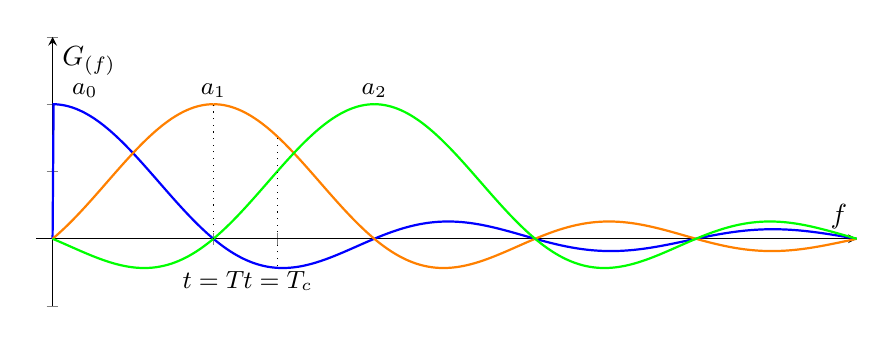
\begin{tikzpicture}
                    \begin{axis}[
                        xlabel=$f$,
                        ylabel=$G_{(f)}$,
                        xmin=-0.1,
                        xmax=5,
                        ymin=-0.5,
                        ymax=1.5,
                        ytick = {},
                        yticklabels = {},
                        xtick={1,1.4},
                        xticklabels={$t=T$,$t=T_c$},
                        axis lines=middle,
                        domain=0:5,
                        xticklabel style = {yshift=-6pt,font = \small}, 
                        samples=800,
                        width=12cm,
                        height=5cm
                    ]
                    \node [] at (0.2,1.1) {\small$a_0$};
                    \node [] at (1,1.1) {\small$a_1$};
                    \node [] at (2,1.1) {\small$a_2$};
                    \addplot [blue, thick, samples = 800,domain = 0:5] {sin(deg(x*pi))/(x*pi)};
                    \addplot [orange, thick, samples = 800,domain = 0:5] {sin(deg((x-1)*pi))/((x-1)*pi)};
                    \addplot [green, thick, samples = 800,domain = 0:5] {sin(deg((x-2)*pi))/((x-2)*pi)};
                    \addplot [black, dotted] coordinates{(1,0)(1,1)};
                    \addplot [black, dotted] coordinates{(1.4,-0.2 )(1.4,0.75)};
                \end{axis}
                \end{tikzpicture}
            \end{figure}
            se non campiono piú a $T$ ma a $T_c$ avró ISI. Per risolvere tali problemi si introduce l'impulso a coseno rialzato.
            
    \subsection{Impulso a coseno rialzato}
        Abbiamo visto come l'impulso rettangolare sia perfetto per soddisfare le Condizioni di Nyquist (\ref*{Condizioni di Nyquist}),
        in generale non viene realizzato tale impulso:
        \begin{itemize}
            \item {Non é facilmente implementabile vista la discontinuitá che $G_{(f)}$ presenta in $f=\pm \frac{1}{2T}$}
            \item {Ha lobi molto pronunciati nel dominio del tempo rendendo il sistema molto sensibile a errori di Sincronizzazione \ref{Errore Sincronizzazione}}
        \end{itemize}
        per rimediare a tali problemi si utilizzano gli impulsi a coseno rialzato o detti Raised Cosine Roll-off (RCR). Essi 
        costituiscono una famiglia di impulsi caratterizzati da un paramentro $\alpha\in [0,1]$ detto \emph{fattore di Roll-off}.
        La trasformata di Fourier si presenta cosí 
        \[
            G_{RCR} = 
            \begin{cases}
                T &|f| \leq \frac{1-\alpha}{2T}\nonumber \\
                \frac{T}{2} \left[1+cos\left(\frac{\pi T}{\alpha}\left[|f| - \frac{1-\alpha}{2T}\right]\right)\right] &\frac{1-\alpha}{2T}<|f|\leq \frac{1+\alpha}{2T}\nonumber \\
                0 &Altrove\nonumber
            \end{cases}    
        \]
        una parte piatta di valore $T$ che si estende fino alla frequenza $\pm \frac{1-alpha}{2T}$. Dopo la parte piatta
        segue una zona di Roll-off che si estende nell'intervallo $\frac{1-alpha}{2T}< f \leq \pm \frac{1+alpha}{2T}$ fino a scendere 
        a $0$. A $f=\frac{1}{2T}$ il valore é sempre indipendente da $\alpha$: $G_{RCR(f)} = \frac{T}{2}$, mentre al variare di $\alpha$:
        \[
            G_{RCR} = 
            \begin{cases}
                \alpha = 0 &\text{É una rect } B_{\alpha=0}=\frac{1}{2T} \nonumber\\
                \alpha=1 &\text{É un triangolo } B_{\alpha=1}=\frac{1}{T}\nonumber\\
                \alpha\neq \{0,1\} & Altro\nonumber
            \end{cases}
        \]
        \begin{figure}[H]
            \centering
            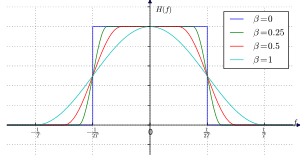
\includegraphics[width = 8cm]{media/Hf-Raised-cosine_filter.png}
            \caption{Funzione coseno rialzato: $G_{RCR(f)}$}
        \end{figure}
        all'aumentare di $\alpha$ la banda di nel dominio del tempo il coseno rialzato ha la forma
        \[
            g_{RCR(t)} = sinc(\frac{t}{T})\frac{cos(\alpha\pi\frac{t}{T})}{1-\frac{2\alpha t}{T}^2}  
        \]
        \begin{figure}[H]
            \centering
            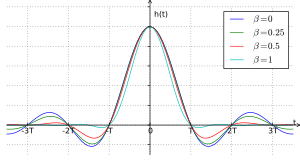
\includegraphics[width = 8cm]{media/ht-Raised-cosine-impulse.png}
            \caption{Funzione coseno rialzato: $g_{RCR(t)}$}
        \end{figure}
        ricordando una $sinc$ ma con lobi molto smorzati man mano che $\alpha$ tende a $1$. 

        Si sceglie il fattore di Roll-off tenendo conto sia della efficenza spettrale che migliora al decrescere di $\alpha$,
        dal dominio del tempo bisogna invece tener conto della sensibilitá all'ISI che diminuisce al crescere di $\alpha$.
        Inoltre una propietá del coseno rialzato é \label{propieta coseno rialzato} 
        \[
            g_{RCR(0)} = \int_{-\infty}^{\infty}G_{RCR(f)}df = 1
        \]
    \subsection{Filtro adattato}
        Ci poniamo adesso il problema del dimensionamento di $g_{(t)}$ in forma estesa, cioé
        dimensionando i filtri $g_{T(t)},g_{R(t)}$ nelle ipotesi che il canale sia $c_{(t)} = \delta_{(t)}$. 
        Il nostro obbiettivo é ridurre al minimo, se non eliminare, sia l'ISI che il rumore, per ottenere ció si introduce
        il fltro adattato (Matched Filter). Il filtro risolve il seguente problema: preso un impulso $p_{(t)}$ di forma nota,
        immerso in rumore additivo bianco $w_{(t)}$ (anche non Gaussiano) con densitá spettrale di potenza $S_{w(f)} = \frac{N_0}{2}$. 
        Il segnale é inviato in ingresso ad un sistema lineare e tempo invariante con risposta impulsiva $h_{(t)}$ e campionato ad un 
        istante $t_{0}$, ottenendo il campione $x_{(t_0)}$ come nel sistema di ricezione
        \begin{figure}[H]
            \centering
            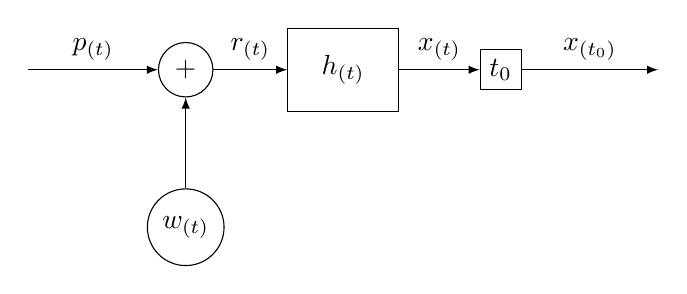
\begin{tikzpicture}[
                    node distance=2cm,
                    >=latex
                ]
                % Blocks
                \node [coordinate,draw] (in) {};
                \node [circle, draw,right of=in] (TX) {$+$};
                \node [circle, draw,below of=TX] (WT) {$w_{(t)}$};
                \node [rectangle, draw,minimum height=3em, minimum width=4em,right of=TX] (C) {$h_{(t)}$};
                \node [rectangle, draw,minimum height=1em, minimum width=1em,right of=C] (RX) {$t_0$};
                \node [coordinate,right of = RX] (output) {};
            
                % Connections
                \draw [->] (in) --node[above]{$p_{(t)}$} (TX);
                \draw [->] (WT) -- (TX);
                \draw [->] (TX) --node[above]{$r_{(t)}$} (C);
                \draw [->] (C) --node[above]{$x_{(t)}$} (RX);
                \draw [->] (RX) --node[above]{$x_{(t_0)}$} (output);
            \end{tikzpicture}
        \end{figure}        
        Volgiamo quindi determinare $h_{(t)}$ in modo che sia massimo il rapporto segnale/rumore (SNR) sul campione $x_{t_0}$. Abbiamo 
        nel sistema
        \begin{gather}
            x_{(t)} = p_{(t)}\otimes h_{(t)}+w_{(t)}\otimes h_{(t)} = s_{(t)}\otimes n_{(t)}\nonumber \\
            \eval*{x_{(t)}}_{t=t_0} = s_{(t_0)} + n_{(t_0)}\nonumber
        \end{gather}
        esplicitando i valori
        \begin{gather}
            s_{(t_0)} = \int_{-\infty}^{\infty} h_{\tau} p_{(t_0-\tau)}d\tau \nonumber\\
            n_{(t_0)} = \int_{-\infty}^{\infty} h_{\tau} w_{(t_0-\tau)}d\tau \nonumber
        \end{gather}
        ricordiamo che $n_0$ é una variabile aleatoria e calcolando l'SNR:
        \[
            \frac{S_u}{N_u} = \frac{s^2_{t_0}}{\mathbb{E}[n^2_{(t_0)}]}  
        \]
        dove 
        \begin{align}
            \mathbb{E}[n^2_{(t_0)}] &= R_{n(0)} \overset{TCF}{=} S_{n(f)} = S_{w(f)}\left|H_{(f)}\right|^2 = \frac{N_0}{2}\left|H_{(f)}\right|^2 \nonumber \\
                                    &\overset{ATCF}{=} \int_{-\infty}^{\infty} S_{n(f)} df = \int_{-\infty}^{\infty} \frac{N_0}{2}\left|H_{(f)}\right|^2 df \nonumber            
        \end{align}
        essendo $H_{(f)}$ la trasformata di fourier di $h_{(t)}$ e tenendo conto del teorema di Parseval ho
        \[
            \mathbb{E}[n^2_{(t_0)}] = \frac{N_0}{2}\int_{-\infty}^{\infty} h_{(t)}^2 dt
        \]
        invece calcolando $s^2_{(t_0)}$ lo dobbiamo scegliere $h_{(t)}$ per massimizzare l'SNR e ridurre al minimo l'errore
        \begin{align}
            SNR &= \frac{s^2_{t_0}}{\frac{N_0}{2}\int_{-\infty}^{\infty} h_{(t)}^2 dt} = \frac{\int_{-\infty}^{\infty} h_{\tau} p_{(t_0-\tau)}d\tau}{\frac{N_0}{2}\int_{-\infty}^{\infty} h_{(t)}^2 dt} \nonumber \\
                &\overset{Dsg. Swartz}{\leq} \frac{\int_{-\infty}^{\infty} h_{\tau}d\tau \int_{-\infty}^{\infty} p_{(t_0-\tau)}d\tau}{\frac{N_0}{2}\int_{-\infty}^{\infty} h_{(t)}^2 dt} = \frac{2}{N_0}E_p \nonumber
        \end{align}        
        l'uguaglianza si ha se $h_{(t)} = kp_{(t_0-t)}$ con $k$ numero reale non nullo, ecco perché si chiama filtro adattato, poiché si adatta all'impulso $p_{(t)}$ e 
        massimizza il rapporto segnale rumore all'istante $t_0$ quando il rumore é bianco e la risposta impulsiva del filtro é 
        \[
            h_{(t)} = p_{(t_0-t)}  
        \]     
        cioé una versione del segnale $p_{(t)}$ ribaltata e traslata di $t_{0}$ come ad esempio 
        \begin{figure}[H]
            \centering
            \subfloat[$p_{(t)}$]{body}
            \hfill
            \subfloat[$p_{(t_0-t)}$]{body}
        \end{figure}
        Si puó ricavare la componente utile del segnale in uscita dal sistema
        \[
            s_{(t_0)} = \int_{-\infty}^{\infty} p{(t_0-t}dt = E_p  
        \]
        e la risposta in frequenza del filtro adattato
        \[
            H_{(f)} = TCF[p_{(t_0-t)}] = P^*_{(f)}e^{-j2\pi ft_0}    
        \]
        con $P_(f) = TCF[p_{(t)}]$. Il modulo del filtro é 
        \[
            \left|H_{(f)}\right| = \left|P_{(f)}\right|   
        \] 
        si osserva come nel domino della frequenza il filtro adattato amplifichi le zone freqeunziali dove $ \left|P_{(f)}\right|$
        é maggiore (zona rapporto segnale rumore elevato) e attenui le zone freqeunziali dove $ \left|P_{(f)}\right|$ é minore 
        (zone a basso rapporto segnale romore), si adatta al segnale.

        \subsubsection{Progettazione dei filtri di ricezione e trasmissione}
            Nella raltá il canale $c_{(t)}$ é un canale distorcente diverso quindi da $\delta_{(t)}$, il dimensionamento di $g_{T(t)}$
            e $g_{R(t)}$. Tipicamente in pratica per il dimensionaemnto di $g_{T(t)}$ e $g_{R(t)}$ consiste nell'assumere il canale 
            come $c_{(t)} = \delta_{(t)}$ in modo tale che quando il canale non é distorcente il segnale venga trasmesso correttamente
            mentre se il canale diventa distorcente si prendereanno delle precauzioni al ricevitore per mitigare tali distorsioni.
            Supponiamo quindi che il canale sia $c_{(t)} = \delta_{(t)}$ gli impulsi in ingresso al filtro di ricezione saranno del tipo
            \[
                g_{TC(t)} = g_{T(t))} \otimes c_{(t)} =  g_{T(t))} 
            \]
            e la risposta impulsiva globale del sistema PAM
            \[
                g_{(t)} = g_{TC(t))} \otimes g_{R(t)} =  g_{T(t))} \otimes g_{R(t)}
            \]
            abbiamo 2 variabili, $g_{T(t)}$ e $g_{R(t)}$, e dobbiamo rispettare 2 condizioni (é un problema di ricerca dell'ottimo):
            \begin{enumerate}
                \item {
                    Annullamento dell'ISI: Dobbiamo fare in modo che $g_{(t)}$ sia un impulso che soddisfi le condizioni di Nyquist,
                    tipicamente un impulso a coseno rialzato
                    \[
                        G_{(f)} = G_{T(f)} \otimes G_{R(f)} = G_{RCR(f)} 
                    \]
                }
                \item {
                    Massimizzare il rapporto Segnale/Rumore sul campionatore in uscita dal filtro di ricezione:
                    si deve fare in modo che il filtro in ricezione $g_{R(t)}$ sia adattato agli impulsi presenti al suo ingresso
                    \[
                        g_{R(t)} = g_{T(-t)} \Rightarrow G_{R(f)} = G_{T(f)}^\ast
                    \]
                    in caso il canale fosse $c_{(t)} \neq \delta_{(t)}$ 
                    \[
                        G_{R(f)} = G_{T(f)}^\ast = \left[G_{T(f)} C_{(f)}\right]^\ast  
                    \]                
                }
            \end{enumerate}
            unendo le due condizioni 
            \[
                G_{RCR(f)} = G_{T(f)}G_{T(f)}^\ast = \left|G_{T(f)}\right|^\ast  
            \]
            dato che la funzione coseno rialzato é reale e non negativa posso esprimere la $G_{T(f)}$ come
            \[
                G_{T(f)} = \sqrt{G_{RCR(f)}} = G_{R(f)}    
            \] 
            cioé le risposte in frequenza dei filtri in trasmissione e ricezione coincidono cone la radice
            quadrata della funzione coseno rialzato. I corrispondenti impulsi nel dominio del tempo 
            $g_{T(t)}$ e $g_{R(t)}$ sono detti \emph{impulsi a radice di coseno rialzato} e con l'acronimo RRCR
            (Root raised cosine Roll-off). Si puó notare come non siano impulsi di Nyquist ma la loro convoluzione 
            invece si.
            \begin{figure}[H]
                \centering
                \subfloat[$g_{RRCR(t)}$]{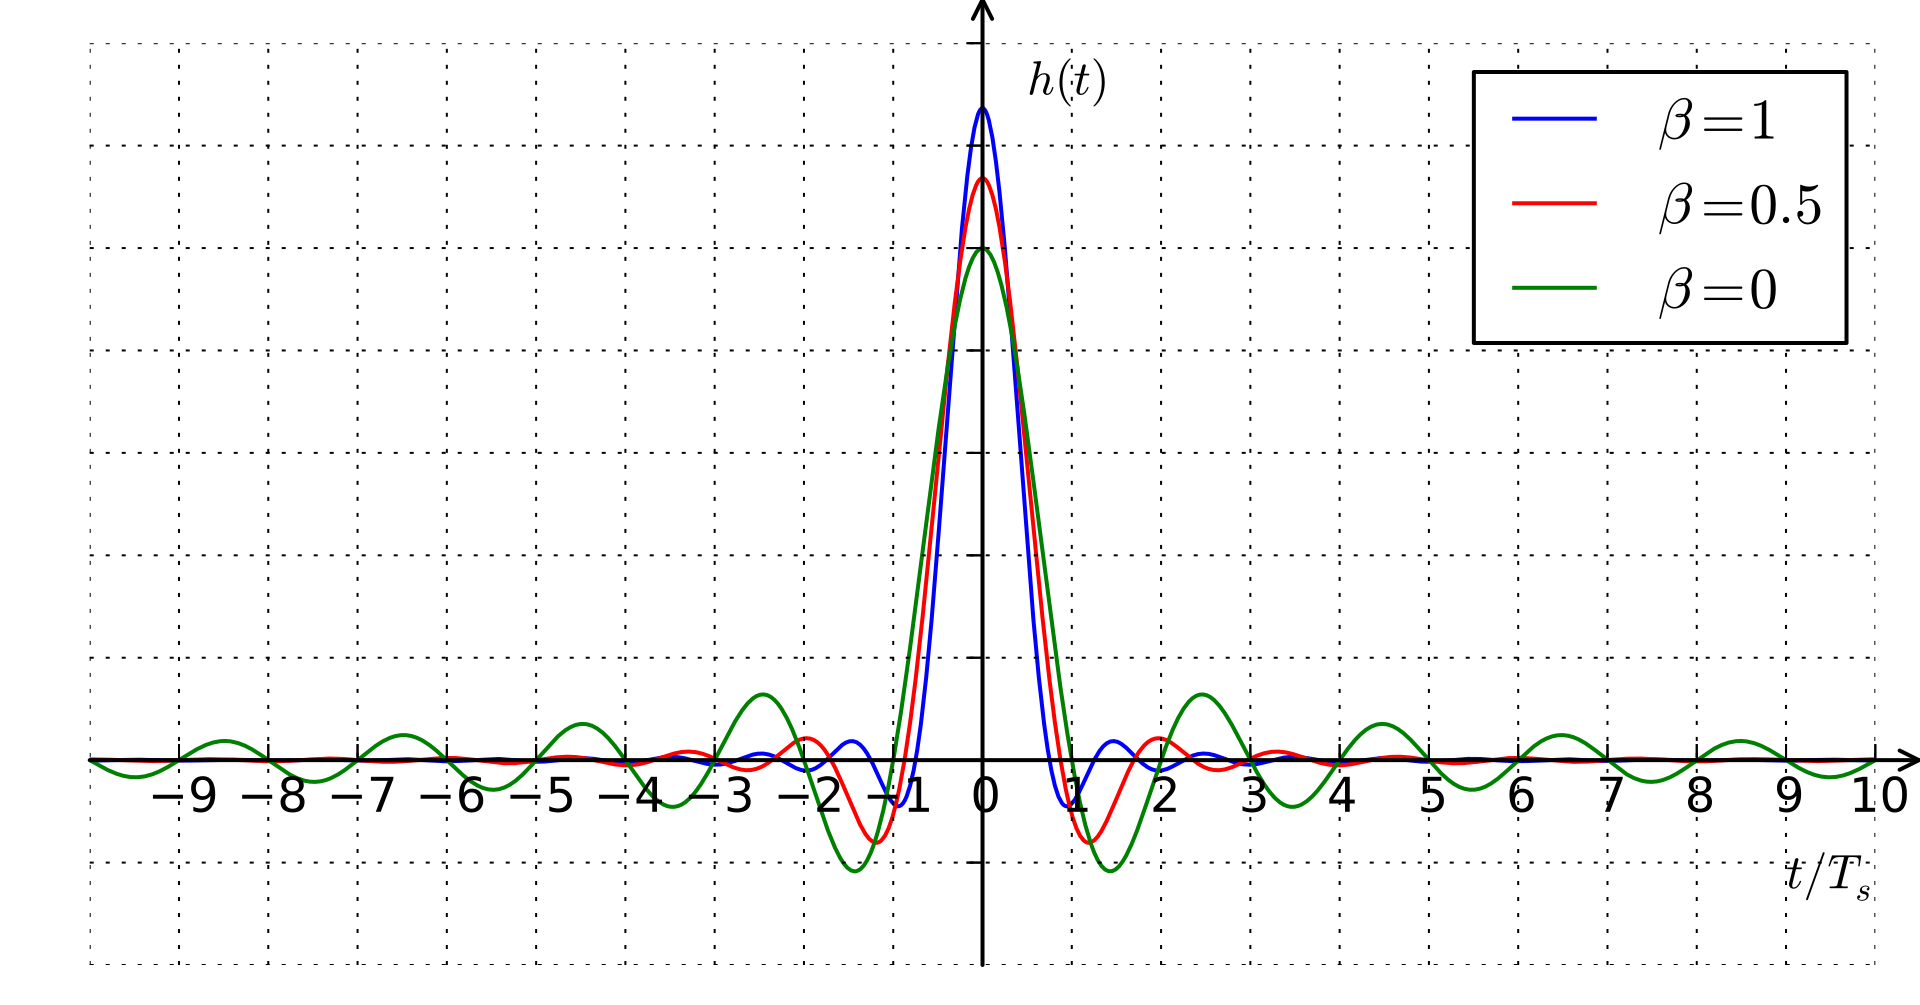
\includegraphics[width = 6cm]{media/Root-raised-cosine-impulse.png}}
                \hfill
                \subfloat[$G_{RRCR(f)}$]{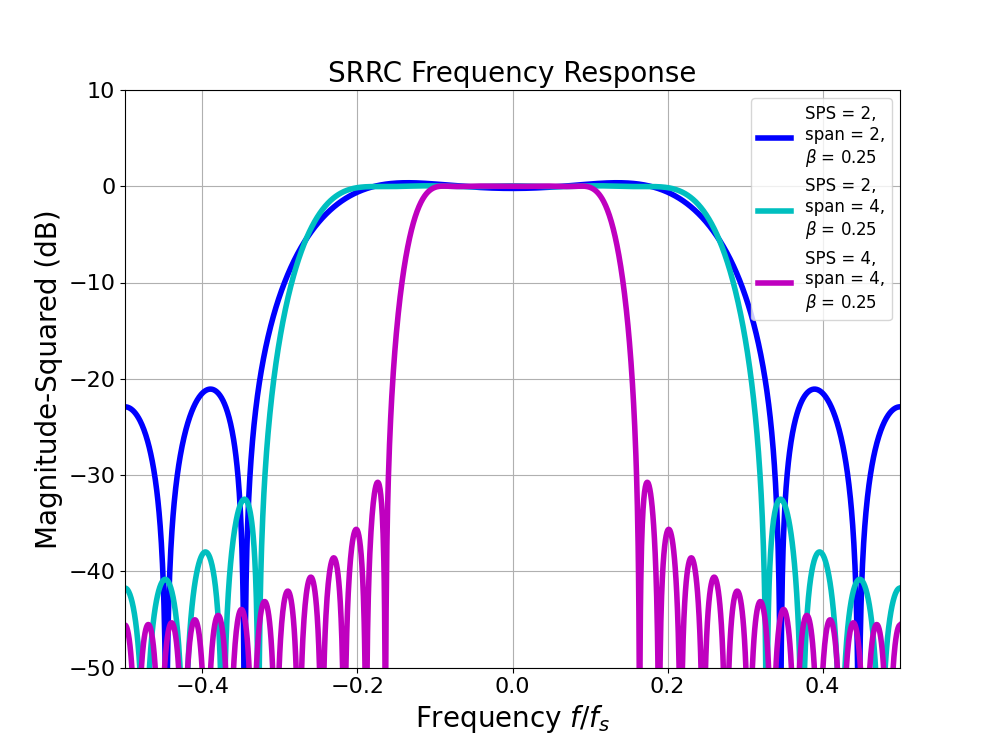
\includegraphics[width = 6cm]{media/srrcDesign_frequencyResponse-1.png}}
            \end{figure}           
            ha gli stessi punti di discesa e valori della funzione a coseno rialzato.
    \subsection{Circuito decisore}
        Siamo giunti al decisore del nostro sistema di comunicazione
        \begin{figure}[H]
            \centering
            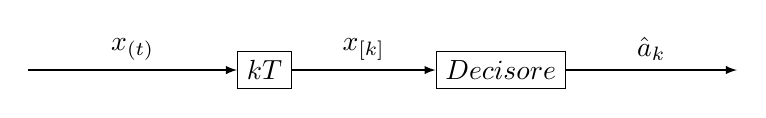
\begin{tikzpicture}[
                    node distance=3cm,
                    >=latex
                ]
                % Blocks
                \node [coordinate,draw] (in) {};
                \node [rectangle, draw,right of=in] (C) {$kT$};
                \node [rectangle, draw,minimum height=1em, minimum width=1em,right of=C] (RX) {$Decisore$};
                \node [coordinate,right of = RX] (output) {};
            
                % Connections
                \draw [->] (in) --node[above]{$x_{(t)}$} (C);
                \draw [->] (C) --node[above]{$x_{[k]}$} (RX);
                \draw [->] (RX) --node[above]{$\hat{a}_{k}$} (output);
            \end{tikzpicture}
        \end{figure}        
        il decisore riceve al suo ingresso il campione $x_{[k]}$ e lo utilizza per prendere una decisioe sul simbolo trasmesso
        $a_k$ usando il criterio di ottimalitá.
        \paragraph{Criterio MAP}
            Il criterio che minimizza la probabilitá di errore sul simbolo $a_k$ é detto criterio MAP (Maximum A-posterior Probability),
            secondo tale criterio il simbolo da scegliere all'interno dell'alfabeto $\mathcal{A} = \{a^{(1)},a^{(2)},\dots,a^{(M)}\}$
            é quello che ha la massimo probabiltá a posteriori di essere stato trasmesso, cioé dopo aver osservato il campione $x_{[k]}$.
            Il criterio MAP sancisce quindi 
            \[
                P_r[a_k = a^{(i)}|x_{[k]}]    
            \]
            la probabilitá di aver trasmesso $\hat{a}_{k}=a^{(i)}$ nell'ipotesi di aver ricevuto $x_{[k]}$, questa sará
            \[
                P_r[a_k = a^{(i)}|x_{[k]}] \leq P_r[a_k = a^{(\ell)}|x_{[k]}]\ \forall i\neq \ell\in \{1,2,\dots,M\}    
            \]
            é minore della probabilitá di scegliere un simbolo $a^{(\ell)}$ sbagliato. Voglio massimizzare la prbabilitá di 
            corretta ricezione 
            \[
                P_r[a_k = a^{(i)}|x_{[k]}] = \frac{f_x[x_{[k]}|a_k = a^{(i)}]P_r[a_k = a^{(i)}]}{f_x[x_{[k]}]}    
            \]
            dove $f_x[x_{[k]}]$ é la funzione densitá di probabilitá del campione $x_{[k]}$,
            é come la probabilitá di Bayes (\ref{Regola di Bayes}) ma con la densitá di probabilitá ($fdp$). Posso analizzare
            solo il numeratore poiché dipende dal simbolo trasmesso, definisco quindi 
            \[
                \gamma_{(a^{(i)},x_{[k]})} = f_x[x_{[k]}|a_k = a^{(i)}]P_r[a_k = a^{(i)}]
            \] 
            ho $\hat{a}_k = a^{(i)}$ se 
            \[
                \gamma_{(a^{(i)},x_{[k]})} > \gamma_{(a^{(\ell)},x_{[k]})}
            \]
            se il numeratore della probabilitá di corretta ricezione é maggiore di quello di sbagliata ricezione, 
            analizzo i due nuemratori nelle ipotesi di 
            \begin{itemize}
                \item {ISI$=0$}
                \item {$c_{(t)} = \delta_{(t)}$ oppure $c_{(t)} = A\delta_{(t-\tau)}$, non cambia tra i due il secondo tipo di canale campiona a $kT+\tau$
                    che é il segnale ritardato}
                \item {$g_{(t)} = g_{TxRCR(t)}\otimes g_{RxRCR(t)} + n_{[k]}$}
            \end{itemize}
            Ho quindi 
            \[
                x_{[k]} \overset{ISI=0}{=} a_kg_{(0)} + n_{[k]} = a_k + (n_{[k]} \sim \mathcal{N}(0,\sigma_n^2))
            \]
            dove 
            \[
                \sigma_n^2 = \int_{-\infty}^{\infty}S_{n(f)}df = \frac{N_0}{2} \int_{-\infty}^{\infty}\underset{\ref{propieta coseno rialzato}}{\left| G_{R(f)} \right|} df = \frac{N_0}{2}  
            \]
            e la funzione densitá di probabiltiá 
            \begin{gather}
                f_x[x_{[k]}|a_k = a^{(i)}] = \frac{1}{\sqrt{2\pi}\sigma_n}e^{\left(\displaystyle -\frac{(x_{[k]}-a^{(i)})^2}{2\sigma_n^2}\right)} \nonumber \\
                x_{[k]} | a_k = a^{(i)} \sim \mathcal{N}(a^{(i)},\sigma_n^2)\nonumber \\
                f_x[x_{[k]}|a_k = a^{(i)}] = \Gamma_{(a^{(i)},x_{[k]})} \nonumber
            \end{gather}
            massimizziamo adesso $\gamma_{(a^{(i)},x_{[k]})}$ con l'ipotesi che i simboli siano equiprobabili $P_r[a^{(i)}] = \frac{1}{M}$. Allora nache il termine
            $P_r[a_k = a^{(i)}]$ diventa trascurabile per la massimizzazione, ne rimane quindi solo da massimizzare
            \[
                \Gamma_{(a^{(i)},x_{[k]})} > \Gamma_{(a^{(\ell)},x_{[k]})}    
            \]
            essendo funzioni monotone decrescenti posso farne il logaritmo naturale
            \begin{gather}
                ln\left(\Gamma_{(a^{(i)},x_{[k]})} \right)> ln\left(\Gamma_{(a^{(\ell)},x_{[k]})}\right) \nonumber\\
                \frac{-\left(x_{[k]}-a^{(i)}\right)^2}{2\sigma_n^2}-ln\left(\sqrt{2\pi}\sigma_n\right) >  \frac{-\left(x_{[k]}-a^{(\ell)}\right)^2}{2\sigma_n^2}-ln\left(\sqrt{2\pi}\sigma_n\right)\nonumber \\
                \left(x_{[k]}-a^{(i)}\right)^2<\left(x_{[k]}-a^{(\ell)}\right)^2\nonumber    
            \end{gather}
            il risultato trovato é la distanza euclidea del simbolo ricevuto minore della distanza euclidea da qualsiasi altro simbolo. Se
            questa disuguaglianza é vera, é il criterio chiamato a distanza minima euclidea o a massima verosomiglianza, valido solo se i simboli
            sono equiprobabili. Ho due criteri 
            \[
                MAP \overset{\text{Se equiprobabili}}{\Rightarrow} \text{Massima verosomiglianza}  
            \] 
            nel caso MAP massimizzo la funzione $\gamma_{(a^{(i)},x_{[k]})}$, nel caso a massima verosomiglianza massimizzo la $\Gamma_{(a^{(i)},x_{[k]})}$ 
            In caso di simboli non equiprobabili si arriva alla funzione 
            \[
                \Gamma_{(a^{(i)},x_{[k]})} = \left[x_{[k]}-a^{(i)}\right]^2-2\sigma^2ln(P_i)
            \]
            con $P_i$ probabilitá a priori del simbolo $a^{(i)}$
        \subsubsection{Zone di decisione}
            Il criterio MAP suddivide l'asse reale in \emph{zone di decisione}, ciascuna associata a un determinato simbolo dell'alfabeto $\mathcal{A}$.
            Indichiamo con $\mathcal{Z}^{(m)}$ la zona di decisione associata al simbolo $a^{(m)}\in\mathcal{A}$, essa é definita come
            \[
                \mathcal{Z}^{(m)} = \left\{ x\in\mathbb{R}: \Gamma_{(a^{(m)},x_{[k]})}<\Gamma_{(a^{(\ell)},x_{[k]})}, a^{(\ell)}\in\mathcal{A} \vee a^{(\ell)}\neq a^{(m)} \right\}
            \]   
            per cui la decisione $\hat{a}_{k}$ viene presa a favore del simbolo $a^{(i)}$ solo se $x_{[k]}\in \mathcal{Z}^{(i)}$. Il decisore altro non é 
            che un comparatore di $x_{[k]}$ con delle soglie in modo da individuare la zona di decisione di $x_{[k]}$. 
            \paragraph{Esempio PAM $\mathcal{A} = \{-1,+1\}$}{
                Prendiamo in esempio una PAM con alfabeto $\mathcal{A} = \{-1,+1\}$ e sia 
                \[
                    p=P_r[a_k=-1]\ e\ 1-p=P_r[a_k=+1]
                \]
                scegliamo il decisore sulla base del criterio MAP e ipotizziamo di dover scegliere per il simbolo $\hat{a}_k =+1$ se
                \[
                    \Gamma_{(+1,x_{[k]})} < \Gamma_{(-1,x_{[k]})} 
                \]  
                svolgendo i calcoli nel caso di simboli non equiprobabili
                \begin{gather}
                    \left[x_{[k]}-1\right]^2-2\sigma^2ln(1-p)<\left[x_{[k]}+1\right]^2-2\sigma^2ln(p)\nonumber \\
                    x_{[k]}> \frac{\sigma^2}{2}ln\left(\frac{p}{1-p}\right) = \lambda\nonumber
                \end{gather}
                \begin{figure}[H]
                    \centering
                    \begin{tikzpicture}
                        \begin{axis}[
                            xlabel=$x$,
                            % ylabel=$\lambda=\frac{\sigma^2}{2}ln\left(\frac{p}{1-p}\right)$,
                            xmin=-3,
                            xmax=3,
                            ymin=-1,
                            ymax=1.3,
                            % ytick = {},
                            % yticklabels = {},
                            xtick={-1.5,1.5},
                            xticklabels={$-1$,$+1$},
                            axis x line=middle,
                            axis y line=none,
                            domain=3:3,
                            samples=800,
                            width=12cm,
                            height=5cm
                        ]
                            \node [] at (-1.5,0.5) {\small\text{Zona di decisione }$\hat{a}_k =-1$};
                            \node [] at (1.5,0.5) {\small\text{Zona di decisione }$\hat{a}_k =+1$};
                            \node [] at (0.8,1) {\small$\lambda=\frac{\sigma^2}{2}ln\left(\frac{p}{1-p}\right)$};
                            \addplot [orange,thick, dotted] coordinates{(0,-1)(0,1.5)};

                        \end{axis}
                    \end{tikzpicture}
                    \caption{Zone di decisione PAM $\mathcal{A} = \{-1,+1\}$}
                \end{figure}
                l'asse é stato suddiviso in due zone di decisione e la soglia $\lambda$ dipende da $\sigma^2$ e $p$.
                Possiamo anche analizza l'andamento di $\lambda$ al variare di $p$ fissato un valore di $\sigma$
                \begin{figure}[H]
                    \centering
                    \begin{tikzpicture}
                        \begin{axis}[
                            xlabel=$p$,
                            ylabel=$\lambda$,
                            xmin=-0.1,
                            xmax=1.5,
                            ymin=-3,
                            ymax=3,
                            ytick = {},
                            yticklabels = {},
                            xtick={0.5,1},
                            xticklabels={$\frac{1}{2}$,$1$},
                            axis lines=middle,
                            domain=0:5,
                            samples=800,
                            width=8cm,
                            height=10cm
                        ]
                        \addplot [black, const plot, thick,samples=1200] {0.5*ln(x/(1-x))};
                        \addplot [orange, dotted, thick] coordinates{(1,-3)(1,3)};
                    \end{axis}
                    \end{tikzpicture}
                \end{figure}
                come si vede nel caso di simboli equiprobabili $p=\frac{1}{2}$ la soglia vale $\lambda=0$, mentre
                assume valori positivi se la probabilitá del simbolo $\hat{a}_k = -1$ é $p>\frac{1}{2}$ ha maggiore 
                probabilitá a priori di essere trasmesso. Il decisore tende a privilegiare la decisione sul simbolo
                che ha maggiore probabilitá a priori di essere trasmesso, allargandone opportunemante la relativa
                zona di decisione.
            }
            
            Consideriamo il caso pratico in cui i simboli dall'alfabeto $\mathcal{A} = \{a^{(1)},\dots,a^{(M)}\}$ siano
            equiprobabili
            \[
                P_m=\frac{1}{M}\ m=1,\dots,M  
            \]
            in questo caso il termine $-2\sigma^2ln(P_m)$ non dipende da $a^{(m)}$ e diventa trascurabile per la decisione
            di $a_k$, il criterio di decisione si riduce alle distanze euclidee e il criterio a \emph{massima verosomiglianza}, $\hat{a}_k=a^{(i)}$ se
            \[
                \Gamma_{(a^{i},x_{[k]})} < \Gamma_{(a^{(\ell)},x_{[k]})}                    
            \]
            che diventano 
            \[
                \left(x_{[k]}-a^{(i)}\right)^2<\left(x_{[k]}-a^{(\ell)}\right)^2  
            \]
            in caso di simboli equiprobabili possiamo notare che le soglie di decisione siano posizionate esattamente a 
            metá tra i due simboli adiacenti dell'alfabeto, ad esempio in un sistema PAM quaternario
            \begin{figure}[H]
                \centering
                \begin{tikzpicture}
                    \begin{axis}[
                        xlabel=$x$,
                        % ylabel=$\lambda=\frac{\sigma^2}{2}ln\left(\frac{p}{1-p}\right)$,
                        xmin=-5,
                        xmax=5,
                        ymin=-1,
                        ymax=1,
                        % ytick = {},
                        % yticklabels = {},
                        xtick={-3,-1,1,3},
                        xticklabels={$-3$,$-1$,$+1$,$+3$},
                        axis x line=middle,
                        axis y line=none,
                        domain=5:5,
                        samples=100,
                        width=12cm,
                        height=5cm
                    ]
                        \node [] at (-1,0.5) {\small$\hat{a}_k =-1$};
                        \node [] at (-3,0.5) {\small$\hat{a}_k =-3$};
                        \node [] at (1,0.5) {\small$\hat{a}_k =+1$};
                        \node [] at (3,0.5) {\small$\hat{a}_k =+3$};
                        \addplot [orange,thick, dotted] coordinates{(0,-1)(0,1)};
                        \addplot [orange,thick, dotted] coordinates{(2,-1)(2,1)};
                        \addplot [orange,thick, dotted] coordinates{(-2,-1)(-2,1)};
                    \end{axis}
                \end{tikzpicture}
                \caption{Zone di decisione 4-PAM $\mathcal{A} = \{-3,-1,+1,+3\}$}
            \end{figure}
            il simbolo deciso dall'alfabeto $\mathcal{A}$ sará pertanto quello che ha distanza euclidea minore rispetto al 
            campione $x_{[k]}$ ricevuto. Il criterio a massima verosomiglianza quindi minimizza l'errore in caso 
            di simboli equiprobabili e a discapito della conoscenza di $\sigma$ e la probabilitá dei simboli,
            possiamo anche utilizzarlo in caso di simboli non equiprobabili fornendoci una soluzione sub-ottima. 
        \subsubsection{Calcolo della SER per un sistema PAM M-ario}
            Consideriamo un sistema PAM con alfabelt M-ario
            \[
                \mathcal{A} = \{\pm 1,\pm 3,\dots, \pm(M-1)\}  
            \]
            il sistema M-PAM ottiene $x_{[k]} = Aa_k + n_{[k]}$,
            vogliamo calcolare la probabilitá media di errore sul simbolo deciso ammettendo che i simboli 
            siano equiprbabili, in assenza di ISI all'ingresso del ricevitore cosí fatto
            \begin{figure}[H]
                \centering
                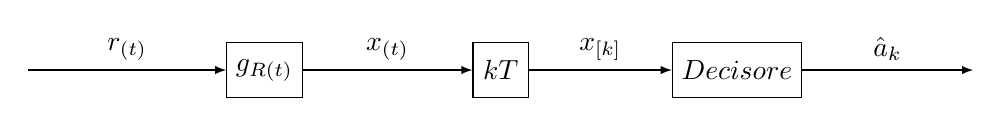
\begin{tikzpicture}[
                        node distance=3cm,
                        >=latex
                    ]
                    % Blocks
                    \node [coordinate,draw] (in) {};
                    \node [rectangle, draw,minimum height=2em, minimum width=2em,right of=in] (C) {$g_{R(t)}$};
                    \node [rectangle, draw,minimum height=2em, minimum width=2em,right of=C] (camp) {$kT$};
                    \node [rectangle, draw,minimum height=2em, minimum width=2em,right of=camp] (RX) {$Decisore$};
                    \node [coordinate,right of = RX] (output) {};
                
                    % Connections
                    \draw [->] (in) --node[above]{$r_{(t)}$} (C);
                    \draw [->] (C) --node[above]{$x_{(t)}$} (camp);
                    \draw [->] (camp) --node[above]{$x_{[k]}$} (RX);
                    \draw [->] (RX) --node[above]{$\hat{a}_{k}$} (output);
                \end{tikzpicture}
            \end{figure}                    
            supponiamo che i filtri in trasmissione e ricezione siano entrambi a radice di coseno rialzato. Il problema di questa 
            approssimazione del sistema é che si suppone un canale di trasmissioene $\delta_{(t)}$ quando in realtá si approssima
            meglio con $A\delta_{(t-\tau)}$, dobbiamo quindi campionare a $kT+\tau$ e scalare per $A$, valori che saranno 
            opportunamente ricevuti al momento della sincronizzazione, il sistema diventa 
            \begin{figure}[H]
                \centering
                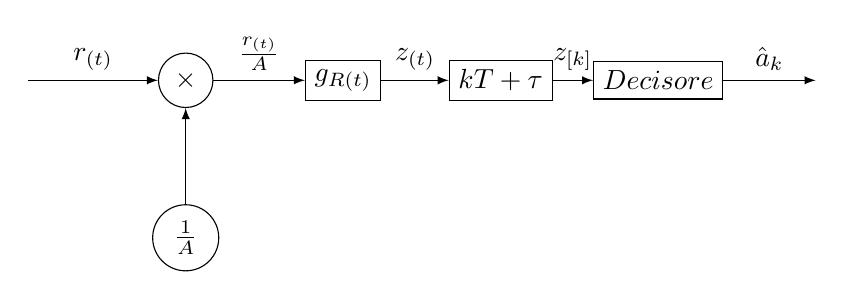
\begin{tikzpicture}[
                        node distance=2cm,
                        >=latex
                    ]
                    % Blocks
                    \node [coordinate,draw] (in) {};
                    \node [circle, draw,right of=in] (scale) {$\times$};
                    \node [circle, draw,below of=scale] (factor) {$\frac{1}{A}$};
                    \node [rectangle, draw,minimum height=1em, minimum width=1em,right of=scale] (C) {$g_{R(t)}$};
                    \node [rectangle, draw,minimum height=1em, minimum width=1em,right of=C] (camp) {$kT+\tau$};
                    \node [rectangle, draw,minimum height=1em, minimum width=1em,right of=camp] (RX) {$Decisore$};
                    \node [coordinate,right of = RX] (output) {};
                
                    % Connections
                    \draw [->] (in) --node[above]{$r_{(t)}$} (scale);
                    \draw [->] (factor) -- (scale);
                    \draw [->] (scale) --node[above]{$\frac{r_{(t)}}{A}$} (C);
                    \draw [->] (C) --node[above]{$z_{(t)}$} (camp);
                    \draw [->] (camp) --node[above]{$z_{[k]}$} (RX);
                    \draw [->] (RX) --node[above]{$\hat{a}_{k}$} (output);
                \end{tikzpicture}
            \end{figure}                    
            dove $z_{[k]} = \frac{x_{[k]}}{A} = a_k + \frac{n_{[k]}}{A}$ il rumore é quindi $\simeq\mathcal{N}(0,\frac{\sigma^2_n}{A^2})$, se calcoliamo
            la varianza nel caso della PAM con simboli indipendenti 
            \[
                \sigma_n^2 = \frac{\sigma^2_n}{A^2} = \frac{N_0}{2}\frac{M^2-1}{3E_s}= \frac{M^2-1}{6(\frac{E_s}{N_0})}    
            \] 
            Se non scalassi per il fattore $A$ le zone di decisione dovrebebro adattarsi al valore di $A$.
            Il decisore suddivide l'asse $x$ in zone di decisione, come mostrato in figura 131, con le soglie poste esattamente
            a metá tra due simboli adiacenti nel caso di simboli equiprobabili
            \begin{figure}[H]
                \centering
                \begin{tikzpicture}
                    \begin{axis}[
                        xlabel=$x$,
                        % ylabel=$\lambda=\frac{\sigma^2}{2}ln\left(\frac{p}{1-p}\right)$,
                        xmin=-6,
                        xmax=6,
                        ymin=-1,
                        ymax=1,
                        % ytick = {},
                        % yticklabels = {},
                        xtick={-5,-3,-1,1,3,5},
                        xticklabels={$-(M-1)$,$-(M-3)$,$\dots$,$\dots$,$M-3$,$M-1$},
                        axis x line=middle,
                        axis y line=none,
                        domain=5:5,
                        samples=100,
                        width=12cm,
                        height=5cm
                    ]
                        \node [] at (-5,0.5) {\small$a^{(1)}$};
                        \node [] at (-3,0.5) {\small$a^{(2)}$};
                        \node [] at (-1,0.5) {\small$\dots$};
                        \node [] at (1,0.5) {\small$\dots$};
                        \node [] at (3,0.5) {\small$a^{(M-1)}$};
                        \node [] at (5,0.5) {\small$a^{(M)}$};
                        \addplot [orange,thick, dotted] coordinates{(0,-1)(0,1)};
                        \addplot [orange,thick, dotted] coordinates{(2,-1)(2,1)};
                        \addplot [orange,thick, dotted] coordinates{(4,-1)(4,1)};
                        \addplot [orange,thick, dotted] coordinates{(-2,-1)(-2,1)};
                        \addplot [orange,thick, dotted] coordinates{(-4,-1)(-4,1)};
                    \end{axis}
                \end{tikzpicture}
                \caption{Zone di decisione M-PAM $\mathcal{A} = \{\pm 1,\pm 3,\dots, \pm(M-1)\}$}
            \end{figure}
            usando il teorema della probabilitá totale possiamo esprimere la SER (Symbol Error Rate)
            \[
                SER = \sum_{i=1}^{M}P[e|a^{(m)}]P_r[a_k=a^{(i)}]    
            \]
            dove 
            \[
                P[e|a^{(m)}] = P_r[\hat{a}_k \neq a_k | a_k=a^{(m)}]
            \]
            nell'ipotesi di simboli equiprobabili
            \[
                SER = \frac{1}{M} \sum_{m=1}^{M}P[e|a^{(m)}]  
            \]
            restan quidi da calcolare le $M$ probabilitá condizionate $P[r|a^{(m)}]$ per $m = 1,\dots,M$.
            L'analisi dell'alfabeto $\mathcal{A}$ e le zone di decisione si puó eveincere come i simboli 
            nelle zone di decisioni esterne ($\pm(M-1)$) abbiano la stessa probabilitá, come anche i 
            simboli interni $\{\pm 1,\dots,\pm (M-3)\}$ abbiano tra di loro la stessa probabilitá. Ne segue che 
            possiamo calcolare solo due probabilitá, ad esempio
            \begin{gather}
                P[e|a^{(m)}] = P[e|a_k = 1]\ se\ a^{(m)\in\{\pm 1,\dots,\pm (M-3)\}}\nonumber \\
                P[e|a_k =-M+1] = P[e|a_k = M-1]\ se\ a^{(m)\in\{\pm (M-1)\}}\nonumber
            \end{gather}
            da cui ricaviamo la SER finale del sistema
            \[
                SER =  \frac{M-2}{M}P[e|a_k = 1]+ \frac{2}{M}P[e|a_k = M-1]
            \]
            dove i coefficenti moltiplicativi sono quanti simboli hanno la relativa probabilitá, ricordiamoci
            che possiamo fare cosí solo perché la costellazione lo permette, magari in casi diversi potrei
            avere piú termini. Il nostro simbolo trasmesso é quindi caratterizzato da
            \[
                z_{[k]} = a_{[k]} + \eta_{[k]}
            \]
            con $\eta_{[k]} = \frac{n_{[k]}}{A} \sim \mathcal{N}(0,\frac{\sigma_n^2}{A^2})\sim \mathcal{N}(0,\sigma_\eta^2)$,
            per un generico simbolo la sua probabilitá di errore é espressa come 
            \[
                P_{err} = Q_{\displaystyle\left(\frac{\lambda - a^{(m)}}{\sigma}\right)}    
            \]
            dove $\lambda - a^{(m)}$ indica la distanza dalla soglia.
            Calcoliamo le probabilitá di errore condizionale:
            \begin{enumerate}
                \item {Calcolo di $P[e|a_k = 1]$
                    Supponiamo sia stato inviato il simbolo $a_k = 1$ il campione ricevuto é 
                    \[
                        z_{[k]} = 1 + \eta_{[k]}  
                    \]
                    \begin{figure}[H]
                        \centering
                        \begin{tikzpicture}
                            \begin{axis}[
                                xlabel=$x$,
                                ylabel=$a$,
                                xmin=-5,
                                xmax=5,
                                ymin=-1,
                                ymax=1,
                                ytick = {},
                                yticklabels = {},
                                xtick={-3,-1,1,3},
                                xticklabels={$\dots$,$-1$,$+1$,$\dots$},
                                axis x line=middle,
                                axis y line=middle,
                                domain=5:5,
                                samples=100,
                                width=12cm,
                                height=5cm
                            ]
                                \node [] at (-1,0.65) {\small$\hat{a}_k =-1$};
                                \node [] at (-3,0.65) {\small$\dots$};
                                \node [] at (1,0.65) {\small$\hat{a}_k =+1$};
                                \node [] at (3,0.65) {\small$\dots$};
                                \addplot [const plot,blue,thick, samples = 300, domain = -4:4] {gauss(1,0.8)};
                                \addplot [const plot,blue,name path = A, samples = 300, domain = -4:0] {gauss(1,0.8)};
                                \addplot [const plot,blue,name path = B, samples = 300, domain = 2:4] {gauss(1,0.8)};
                                \addplot [orange,thick, dotted] coordinates{(0,-1)(0,1)};
                                \addplot [orange,thick, dotted] coordinates{(2,-1)(2,1)};
                                \addplot [orange,thick, dotted] coordinates{(-2,-1)(-2,1)};
                                \addplot [black,const plot,name path = C] coordinates{(2,0)(4,0)};
                                \addplot [black,const plot,name path = D] coordinates{(0,0)(-4,0)};
                                \addplot[red,opacity = 0.3] fill between[of=A and D];
                                \addplot[red,opacity = 0.3] fill between[of=B and C];
                        \end{axis}
                        \end{tikzpicture}
                    \end{figure}
                    notiamo come l'errore é presente quando il simbolo non é compreso all'interno dell'intervallo
                    \begin{align}
                        P[e|a_k =1] &= P_r[z_{[k]}< 0 \cup z_{[k]}> 2] = P_r[1+\eta_{[k]}< 0 \cup 1+\eta_{[k]}> 2] \nonumber \\
                                    &= P_r[\eta_{[k]}< -1 \cup \eta_{[k]}> 1]\nonumber 
                    \end{align}
                    potremmo calcolare l'integrale della distribuzione di probabilitá ma utilizziamo la funzione $Q$,
                    gli intervalli di errore esterni sono uguali quindi possiamo calacolare $Q$ solo nel punto destro
                    \[
                        P[e|a_k =1] = 2Q_{\displaystyle\left(\frac{1}{\sigma_\eta}\right)}  
                    \]
                    
                }
                \item {Calcolo di $P[e|a_k = M-1]$
                    Supponiamo di aver trasmessio il simbolo $a_k = M-1$, il campione é caratterizzato da
                    \[
                        z_{[k]} = M-1+\eta_{[k]}    
                    \]
                    \begin{figure}[H]
                        \centering
                        \begin{tikzpicture}
                            \begin{axis}[
                                xlabel=$x$,
                                ylabel=$a$,
                                xmin=-5,
                                xmax=5,
                                ymin=-1,
                                ymax=1,
                                ytick = {},
                                yticklabels = {},
                                xtick={-3,-1,1,3},
                                xticklabels={$-M+1$,$\dots$,$\dots$,$M-1$},
                                axis x line=middle,
                                axis y line=middle,
                                domain=5:5,
                                samples=100,
                                width=12cm,
                                height=5cm
                            ]
                                \node [] at (-3,0.65) {\small$\hat{a}_k =-M+1$};
                                \node [] at (-1,0.65) {\small$\dots$};
                                \node [] at (3,0.65) {\small$\hat{a}_k =M-1$};
                                \node [] at (1,0.65) {\small$\dots$};
                                \addplot [orange,thick, dotted] coordinates{(0,-1)(0,1)};
                                \addplot [orange,thick, dotted] coordinates{(2,-1)(2,1)};
                                \addplot [orange,thick, dotted] coordinates{(-2,-1)(-2,1)};

                                \addplot [const plot,blue,thick, samples = 300, domain = 0:5] {gauss(3,0.8)};
                                \addplot [const plot,blue,name path = A, samples = 300, domain = 0:2] {gauss(3,0.8)};
                                \addplot [black,const plot,name path = B] coordinates{(0,0)(2,0)};
                                \addplot[red,opacity = 0.3] fill between[of=A and B];
                        \end{axis}
                        \end{tikzpicture}
                    \end{figure}
                    ho errore quando il simbolo non rientra nella semiretta $[M-2,+\infty]$
                    \begin{align}
                        P[e|a_k=M-1] &= P_r[z_{[k]}<M-2] = P_r[M-1+\eta_{[k]}<M-2] = P_r[\eta_{[k]}<-1] \nonumber \\
                                     &= P_r[\eta_{[k]}>1]\nonumber
                    \end{align}
                    dalla figura possiamo ricavare la probabilitá di errore 
                    \begin{align}
                        P[e|a_k=M-1] &= 1-Q_{\displaystyle \left(\frac{\lambda-a^{(m)}}{\sigma_\eta}\right)} = 1-Q_{\displaystyle\left(-\frac{1}{\sigma_\eta}\right)} \nonumber \\
                                     &= Q_{\displaystyle\left(\frac{1}{\sigma_\eta}\right)} \nonumber
                    \end{align}
                }
            \end{enumerate}
            Sostituiendo i risultati ottenuti nella formula della SER
            \begin{align}
                SER &= \frac{M-2}{M}2Q_{\displaystyle\left(\frac{1}{\sigma_\eta}\right)}+ \frac{2}{M}Q_{\displaystyle\left(\frac{1}{\sigma_\eta}\right)} \nonumber \\
                    &= \frac{2(M-1)}{M} Q_{\displaystyle\left(\frac{1}{\sigma_\eta}\right)} \nonumber
            \end{align}
            se la vogliamo esprimere in funzione del valore di $\sigma_\eta= \frac{\sigma_n^2}{A^2} = \frac{N_0}{2A^2}$
            \[
                SER = \frac{2(M-1)}{M} Q_{\displaystyle\left(\sqrt{\frac{2A^2}{N_0}}\right)} 
            \]
            Vogliamo adesso esprimere la SER in funzione dell energia del segnale ricevuto, prendiamo il segnale 
            ricevuto non filtrato 
            \[
                r_{(t)} = S_{R(t)} + w_{(t)} = \sum_{i}Aa_ig_{T(t-iT)}+w_{(t)}    
            \]
            la cui densitá spettrale di potenza é espressa come
            \[
                S_{R(f)} = \frac{A}{T}S_{a(f)}\left|G_{T(f)}\right|^2
            \]
            se i simboli sono independenti ed equiprobabili e sono nel caso di una PAM posso esprimere 
            densitá spettrale di potenza dei simboli come
            \begin{align}
                S_{a(f)} &= \sum_{m}R_{a(m)}e^{-j2\pi fmT} = R_{a(0)}\nonumber \\
                         &= E[a_m^2] = \frac{M^2-1}{3}\nonumber
            \end{align}
             
            allora $S_{R(f)}$ diventa
            \[
                S_{R(f)} = \frac{A}{T}\frac{M^2-1}{3}\left|G_{T(f)}\right|^2
            \]
            dalla quale possiamo calcolare l'energia dei simboli moltiplicando pet $T$ o dei bit 
            moltiplicando per $T_d$ 
            \[
                E_{simboli} = \int_{-\infty}^{\infty}S_{R(f)} df \overset{\ref{propieta coseno rialzato}}{=} A^2\frac{M^2-1}{3}  
            \]
            $A$ puó essere quindi espresso in funzione dell'energia dei simboli 
            \[
                A^2 = \frac{3E_{simboli}}{M^2-1} 
            \]  
            la SER espressa tramite l'energia del simbolo ricevuto é
            \[
                SER = \frac{2(M-1)}{M} Q_{\displaystyle\left(\sqrt{\frac{6E_{simboli}}{(M^2-1)N_0}}\right)} 
            \]
            nel caso di una PAM binaria 
            \[
                SER \overset{M=2}{=} Q_{\displaystyle\left(\sqrt{\frac{2E_{simboli}}{N_0}}\right)} 
            \]
        \subsubsection{Efficenza spettrale ed efficenza energetica}
            Abbiamo visto come l'impulso di trasmissione $g_{T(t)}$ impiegato in un sistema PAM sia tipicamente 
            un impulso a Radice di Coseno RIalzato (\ref{F. Coseno Rialzato}). Nel caso di simboli indipendenti
            ed equiprobabili, la densitá spettrale di potenza del segnale trasmesso é 
            \[
                S_{s(f)} = \frac{M^2-1}{3T}\left|G_{T(f)}\right|^2 = \frac{M^2-1}{3T} G_{RCR(f)}
            \]
            per cui la banda impiegata dal segnale PAM é 
            \[
                B_s = \frac{1+\alpha}{2T}
            \]
            e dipende sia dal fattore di Roll-off, $\alpha$, che dalla frequenza di segnalazione $f_s=\frac{1}{T}$
            \paragraph{Efficenza Spettrale: }\index{Efficenza Spettrale}\label{Efficenza Spettrale} l'efficenza spettrale del sistema PAM é definita da 
                \[
                    \eta_{sp} = \frac{R_d}{B_T} [\frac{bit}{Hz}]    
                \]
                dove $R_d=\frac{log_2(M)}{T}$ é il bit-rate, ho quindi nel caso di impulsi $RCR$ 
                nella PAM
                \[
                    \eta_{sp} = \frac{2log_2(M)}{1+\alpha} [\frac{bit}{Hz}]    
                \]
                questo indica come l'efficenza spettrale del sistema aumenta al crescere della cardinalitá $M$
                dell'alfabeto. 
            \paragraph{Efficenza Energetica: }\index{Efficenza Energetica}\label{Efficenza Energetica}
                Per valutare l'efficenza energetica del sistema occorre analizzare le curve della SER 
                al variare del rapporto $\frac{E_{simboli}}{N_0}$.
                \begin{figure}[H]
                    \centering
                    \includegraphics*[width = 8cm]{media/uwu.png}
                    \caption{Scala logaritmica SER}
                \end{figure}
                La SER é espressa in scala logaritmica ed il rapporto $\frac{E_{simboli}}{N_0}$ é espresso in $db$.
                Viene solitamente fissata una probabilitá di errore obbiettivo stabilita in base all'applicazione, il
                rapporto $\frac{E_{simboli}}{N_0}$ richiesto per raggiungere la SER obbiettivo cresce al crescere della 
                cardinalitá $M$. Questo riduce come l'efficenza energetica del sistema diminuisca al crescere di $M$, entra piú rumore.
                Concludiamo che la scelta dell'alfabeto $\mathcal{A}$ é vincolata da due esigenze contrastanti:
                da un lato sarebbe bene scegliere una carinalitá $M$ elevata per aumentarne l'efficenza spettrale, dall'altro
                lato la scelta di un valore $M$ elevato peggiora l'efficenza energetica del sistema.
            \paragraph{Perdita Energetica: } Si definisce perdica energetica di un sistema di comunicazione numerico $A$ rispetto
                ad un sistema $B$ l'aumento (in $db$) del rapporto $\frac{E_{simboli}}{N_0}$ necessario al sistema $A$ per 
                raggiungere la stessa SER del sistema $B$. Un esempio mostrato in figura evince la perdita del sistema 
                4-PAM rispetto al sistema 2-PAM.
                \begin{figure}[H]
                    \centering
                    \includegraphics*[width = 8cm]{media/uwu.png}
                    \caption{differenza log 4PAM e 2PAM}
                \end{figure}  
                Calcoliamo la perdita in modo analitico basta eguagliare le SER della 4-PAM e della
                2-PAM ottenendo
                \[
                    \frac{3}{2}Q_{\displaystyle\left(\sqrt{\frac{4}{5}\left(\frac{E_s}{N_0}\right)_{M=4}}\right)} =Q_{\displaystyle\left(\sqrt{2\left(\frac{E_s}{N_0}\right)_{M=2}}\right)}      
                \]
                solitamente si tende a trascurare eventuali coefficenti moltiplicativi, potendo cosí confrontare direttamente
                l'argomento della funzione $Q$
                \[
                    \frac{4}{5}\left(\frac{E_s}{N_0}\right)_{M=4} =2\left(\frac{E_s}{N_0}\right)_{M=2}          
                \]
                la perdita del sistema 4-PAM rispetto al sistema 2-PAM é in $db$
                \[
                    \eval*{L}_{db} = 10log_{10}\left(\frac{\left(\frac{E_s}{N_0}\right)_{M=4}}{\left(\frac{E_s}{N_0}\right)_{M=2}}\right) = 10log_{10}\left(\frac{5}{2}\right) \simeq 4db    
                \]
                cioé comporta che la curva di SER per la 4-PAM é praticamente la stessa del sistema 2-PAM, salvo una traslazione di
                circa $4db$ verso destra.
            \paragraph{Esempio sistema 4-PAM}{

            }
        \subsubsection{Codifica GRAY nel sistema PAM}
            Abbiamo visto come la SER in un sistema PAM dipende dal rapporto $\frac{E_s}{N_0}$ e dalla cardinalitá 
            $M$ dell'alfabeto $\mathcal{A}$. Come sappiamo i simboli di modulazione $\{a_i\}$ in un sistema PAM sono
            il risultato della mappatura dei bit di codice $\{d_n\}$. Per l'utente finale sarebbe quindi piú utile 
            conoscere al posto della SER la probabilitá di errore sui bit $\{d_n\}$, chiamata Bit Error Rate (BER)
            \[
                BER = P_r[\hat{d}_n \neq d_n]    
            \] 
            in generale il calcolo della BER in un sistema PAM é un valore difficilmente calcolabile poiché oltre a dipendere
            dal rapporto $\frac{E_s}{N_0}$ e da $M$, dipende anche dalla legge di mappatura. É peró possibile 
            individuare facilmente un intervallo di valori entro quale siamo sicuri che si trovi la BER.
            Per individuare tale intervallo, supponiamo di utilizzare una trasmissione PAM usando un alfabeto
            M-ario e siano
            \begin{gather}
                N_s = \text{Numero di simboli trasmessi}\nonumber \\
                N_d = \text{Numero di bit trasmessi}\nonumber \\
                N_{se} = \text{Numero di simboli ricevuti errati}\nonumber \\
                N_{de} = \text{Numero di bit ricevuti errati}\nonumber 
            \end{gather}
            Si tenga presente che ogni simbolo PAM é ottenuto mappando un blocco di $log_2(M)$ bit, ho quindi
            \[
                N_d = N_slog_2(M)    
            \]
            inoltre ogni volta che un simbolo viene ricevuto con errore il numero dei corrispondenti bit sbagliati 
            varia da $1$ a $log_2(M)$. Si ha pertanto 
            \[
                N_{se} \leq N_{de} \leq N_{se} log_2(M)    
            \]
            dividendo i termini della precedente relazione per $N_d$ si trova
            \[
                \frac{N_{se}}{N_slog_2(M)} \leq \frac{N_{de}}{N_{d}} \leq \frac{N_{se} log_2(M)}{N_{s} log_2(M)}    
            \]
            e passando al limite per $N_s$ e $N_b$ tendendo all'infinito 
            \[
                \frac{SER}{log_2(M)} \leq BER \leq SER    
            \]
            da cui si vede che la BER non puó mai superare la SER. A seconda della legge di mappatura impiegata,
            la BER puó assumere valori piú vicini a $\frac{SER}{log_2(M)}$ o a SER. Vale la pena notare che la BER 
            coinciderebbe con il valore $\frac{SER}{log_2(M)}$ solo se, ogni volta che un simbolo ricevuto contiene 
            un errore, sol uno dei bit corrispondenti a quel simbolo é sbagliato. Questa osservazione é utile 
            per individuare quale sia la mappa ottima. Infatti, tenendo conto che quando un simbolo é ricevuto con errore
            molto probabilmente viene frainteso con un simbolo adiacente nell'alfabeto $\mathcal{A}$, la mappa ottima é 
            quella che associa a simboli adiacenti di $\mathcal{A}$ blocchi di $log_2(M)$ bit che differiscono per un solo bit. 
            Una tale mappa é nota come "Mappa GRAY", ed é quella che minimizza la BER per un prefissato valore della SER. 
            Se in un sistema PAM viene utilizzata la mappadi GRAY, la BER é espressa da 
            \[
                BER \simeq \frac{2(M-1)}{Mlog_2(M)}Q_{\displaystyle \left(\sqrt{\frac{6log_2(M)}{M^2-1}}\frac{E_d}{N_0}\right)}    
            \] 
    \subsection{QUAM}
        É un sistema di comunicazione in {\color{red}banda passante} in cui il segnale trasmesso $s_{T(t)}$ ha densitá 
        spettrale di potenza di tipo passa-banda, centrate su una frequenza $f_0$ detta frequenza portante.
        \subsubsection{Inviluppo complessso}
            l'inviluppo complesso del segnale trasmesso é 
            \[
                \tilde{s}_{(t)} = I_{(t)} +j Q_{(t)}      
            \]
            e il segnale trasmesso
            \[
                  s_{T(t)} = \mathbb{R}e\{\tilde{s}_{(t)}e^{j\omega_0t}\}
            \]
            con $\omega_0 = 2\pi f_0$, $\tilde{s}_{(t)}\in \mathbb{C}$, $I_{(t)}\in \mathbb{R}$ detta parte in fase e 
            $Q_{(t)}\in \mathbb{R}$ detta parte in quadratura del segnale $s_{T(t)}$ il quale puó quindi essere espresso 
            come 
            \[
                s_{T(t)} =I_{(t)}\cos(\omega_0t)+jQ_{(t)}\sin(\omega_0t)  
            \]  
            e le singole parti possono essere espresse come 
            \begin{gather}
                I_{(t)} = \sum_{i}a_ig_{T(t-iT)}\nonumber \\
                Q_{(t)} = \sum_{i}b_ig_{T(t-iT)}\nonumber
            \end{gather}
            in cui $g_{T(t)}$ é l'impulso di trasmissione, $T$ é l'intervallo di segnalazione,
            $\{a_i\}$ e $\{b_i\}$ sono i simboli di modulazione, ottenuti dal mappaggio di bit del codice $\{d_n\}$.
            La mappa ha cardinalitá $M$ ed é di tipo bidimensionale, nel senso che ad ogni stringa di $log_2(M)$ bit di codice
            fa corrispondere una coppia $(a_i,b_i)$ disponibili nell'alafabeto impiegato. $M$ é il numero possibile di coppie $(a_i,b_i)$ 
            disponibili nell'alfabeto. Nel caso di mappe bidimensionali l'alfabeto é costituito da punti $(a_i,b_i)$ nel iano cartesiano,
            ed é detto \emph{costellazione}. Un esempio di costellazione quaternaria é mostrata nella figura seguente
            \begin{figure}[H]
                \centering
                \includegraphics*[width = 8cm]{media/uwu.png}
                \caption{Costellazione quaternaria}
            \end{figure}
        \subsubsection{Trasmettitore - QUAM}
            Il trasmettitore usa un modulatore $I/Q$ come illustrato di seguito, dove $g_{T(t)}$ é un impulso a radice di coseno rialzato 
            come quello impiegato in un sistema PAM.
            \begin{figure}[H]
                \centering
                \includegraphics*[width = 8cm]{media/uwu.png}
                \caption{Trasmettitore QUAM}
            \end{figure}
            L'inviluppo complesso del segnale trasmesso é espresso da
            \[
                \tilde{s}_{(t)} = I_{(t)} +jQ_{(t)} = \sum_{i}c_ig_{T(t-iT)}
            \]
            avendo definito i simboli complessi come 
            \[
                c_i = a_i+jb_i    
            \]
            e si vede che $\tilde{s}_{(t)}$ é in pratica un segnale PAM con simboli complessi. L'equivalente in banda base del trasmettitore é 
            \begin{figure}[H]
                \centering
                \includegraphics*[width = 8cm]{media/uwu.png}
                \caption{Equivalente in Banda Base}
            \end{figure}
        \subsubsection{Densitá spettrale di potenza - QUAM}
            Per il calcolo della densitá spettrale di potenza del segnale $s_{T(t)}$, si ricorda che essa é legata a quella dell'inviluppo
            complesso $\tilde{s}_{(t)}$ dalla relazione
            \[
                S_{s(f)} = \frac{1}{4}\left[S_{\tilde{s}{(f-f_0)}}+ S_{\tilde{s}{(-f-f_0)}}\right]    
            \]
            per cui é sufficiente calcolare la densitá spettrale di potenza $S_{\tilde{s}(f)}$. Ammettiamo che la sequenza dei 
            simboli $\{c_i\}$ sia stazionaria in senso lato con valore medio 
            \[
                \eta_c=\mathbb{E}[c_i]    
            \] 
            e funzione di autocorrelazione
            \[
                R_{c(m)} = \mathbb{E}[c_{i+m}c^\ast_i]    
            \]
            la densitá spettrale di potenza di $\tilde{s}_{T(t)}$ é la trasformata di Fourier di $R_{\tilde{s}{(f-f_0)}}$ ed é espressa da
            \[
                S_{\tilde{s}{(f)}} = \frac{1}{T} f_{c(f)}\left|G_{T(f)}\right|^2    
            \]
            dove 
            \[
                f_{c(f)} = \sum_{m}R_{c(m)}e^{-j2\pi fmT}
            \]
            é la densitá spettrale di potenza dei simboli complessi $\{c_i\}$. La potenza di $s_{T(t)}$ é quindi esprimibile come
            \[
                P_s=\frac{1}{2T} \int_{-\infty}^{\infty} f_{c(f)} \left|G_{T(f)}\right|^2 df
            \]
            Poiché $g_{T(t)}$ é un impulso tipicamente a radice di coseno rialzato, la banda di $\tilde{s}_{T(t)}$ é 
            \[
                B_{\tilde{s}}=\frac{1+\alpha}{2T}    
            \]
            la banda del segnale trasmesso $s_{T(t)}$ 
            \[
                B_{T}=2B_{\tilde{s}} =\frac{1+\alpha}{T}
            \]
            e l'efficenza spettrale del sistema risulta 
            \[
                \eta_{sp} = \frac{R_d}{B_T} = \frac{log_2(M)}{1+\alpha} 
            \]
            avendo tenuto conto che $R_d = \frac{log_2(M)}{T}$. Si osservi come l'efficenza spettrale del sistema aumenti all'aumentare 
            della cardinalitá $M$ della costellazione.
        \subsubsection{Ricevitore - QUAM}
            Supponiamo che il canale sia non distorcente ed aggiunga solo rumore termico. In tale ipotesi, il segnale ricevuto 
            é espresso da
            \[
                r_{(t)} = s_{T(t)}+w_{(t)}    
            \]
            con $w_{(t)}$ rumore Gaussiano bianco avente densitá spettrale di potenza $\frac{N_0}{2}$. Il ricevitore ha la
            struttura mostrata in figura seguente 
            \begin{figure}[H]
                \centering
                \includegraphics*[width = 8cm]{media/uwu.png}
                \caption{Ricevitore QUAM}
            \end{figure}            
            Il segnale ricevuto viene inviato a un filtro passa-banda(\ref{Filtro Passa Banda di banda B - Band Pass Filter (BP)})
            con frequenza centrale $f_0$ e tale da non distorcere il segnale utile. Esso serve a selezionare il segnale utile e ad 
            eleminare il rumore fuori banda. Dopo la demodulazione $I/Q$, il segnale passa attraverso il filtro di ricezione $g_{R(t)}$,
            tipicamente a radice di coseno rialzato, che sostituisce il passa-basso presente nel demodulatore di $I/Q$. I segnali 
            $x_{c(t)}$ e $x_{s(t)}$ in uscita dal filtro di ricezione sono espressi da 
            \begin{gather}
                x_{c(t)} = \sum_{i}a_ig_{(t-iT)}+n_{c(t)}\nonumber \\
                x_{s(t)} = \sum_{i}b_ig_{(t-iT)}+n_{s(t)}\nonumber
            \end{gather}
            dove $g_{(t)} = g_{(T(t))}\otimes g_{(R(t))}$ é un impulso a coseno rialzato, mentre $n_{c(t)}$ e $n_{s(t)}$ sono 
            processi di rumore Gaussiano, a media nulla e a densitá spettrale di potenza
            \[
                S_{n_c(f)} = S_{n_s(f)} = N_0\left|G_{R(f)}\right|^2   
            \]
            Qualora il filtro passa-banda sia simmetrico intorno a $f_0$ i processi $n_{c(t)}$ e $n_{s(t)}$ sono anche incorrelati, e quindi 
            indipendenti essendo congiuntamente Gaussiani. Dopo il campionatore abbimo i campioni $x_{c[k]}$ e $x_{s[k]}$ espressi da 
            \begin{gather}
                x_{c[k]} = a_[k]+n_{c[k]}\nonumber \\
                x_{s[k]} = b_[k]+n_{s[k]}\nonumber
            \end{gather}
            dove si é tenuto conto che $g_{(t)}$ sia un impulso di Nyquist. Le variabili aleatorie $n_{c[k]}$ e $n_{s[k]}$ sono 
            Gaussiane, a media nulla con varianza 
            \[
                \sigma^2 = N_0\int_{-\infty}^{\infty}\left|G_{R(f)}\right|^2df= N_0g_{RCR(0)} = N_0
            \]
            l'equivalente in banda base del ricevitore é 
            \begin{figure}[H]
                \centering
                \includegraphics*[width = 8cm]{media/uwu.png}
                \caption{Equivalente ricevitore in banda base}
            \end{figure}
            dove
            \begin{gather}
                \tilde{x}_{[k]} = c_{[k]}+\tilde{n}_{[k]} \nonumber \\
                \tilde{n}_{[k]} = n_{c[k]}+jn_{s[k]} \nonumber 
            \end{gather}
    \subsection{Modulazione Amplitude Shift Keyring - ASK}
        In questo tipo di modulazione, i simboli $b_i$ sono posti a zero, risolta quindi $Q_{(t)} = 0$. 
        Il segnale trasmesso risulta 
        \[
            s_{T(t)} = I_{(t)}\cos(\omega_0 t)
        \]
        dove $I_{(t)}$ é un segnale PAM
        \[
            I_{(t)} = \sum_{i}a_ig_{T(t-iT)}    
        \]
        con simboli $\{a_i\}$ appartenenti all'alfabeto M-ario $\mathcal{A} = \{\pm 1, \pm 3,\dots,\pm (M-1)\}$. Pertanto 
        il segnale ASK non é altro che un segnale PAM traslato in frequenza mediante modulazione classica. Lo schema trasmettitore 
        é riportato in figura 
        \begin{figure}[H]
            \centering
            \includegraphics*[width = 8cm]{media/uwu.png}
            \caption{Trasmettitore ASK}
        \end{figure}        
        e si vede che é composto solo dal ramo relativo a $I_{(t)}$. Nel caso di simboli indipendenti ed equiprobabili, la densitá 
        spettrale di potenza dell'impulso complesso é 
        \[
            S_{\tilde{s}(f)} = \frac{M^2-1}{3T}\left|G_{T(f)}\right|^2
        \]
        e l'energia media per simbolo trasmesso é 
        \begin{align}
            E_s &= \frac{1}{2}T\int_{-\infty}^{\infty}S_{\tilde{s}(f)}df\nonumber \\
                &= \frac{M^2-1}{6}E_{g_T}\nonumber
        \end{align}
        essendo $E_{g_T}$ l'energia di $g_{T(t)}$. Qualora $g_{T(t)}$ sia un impulso a radice di coseno rialzato, l'efficenza spettrale
        del sistema ASK é 
        \[
            \eta_{sp} = \frac{log_2(M)}{1+\alpha}    
        \]
        ed é la metá di quella del corrispondente segnale PAM trasmesso in banda base. Il ricevitore é costituito da un demodulatore seguito da 
        un ricevitore per segnali PAM, secondo quanto riportato nella figura seguente
        \begin{figure}[H]
            \centering
            \includegraphics*[width = 8cm]{media/uwu.png}
            \caption{Ricevitore ASK}
        \end{figure}
        Ricordando che il guadagno di demodulazione é pari a $1$, é facile capire che le prestazioni in termini di SER e BER per un sistema ASK
        M-ario coincidono con quelle di un sistema PAM. In particolare continua a valere che aumentando la cardinalitá $M$ dell'alfabeto 
        si ha una diminuzione dell'efficenza energetica a favore di un aumento in quella spettrale, a paritá di $M$ l'efficenza 
        spettrale del sistema ASK é la metá di quella del corrispondente sistema PAM. 
    \subsection{Modulazione Quadrature Amplitude Modulation - QAM}
        In questo tipo di modulazione, la cardinalitá $M$ della costellazione é una potenza di $4$, e i simboli $\{a_i\}$ e $\{b_i\}$
        vengono generati da due mappe PAM a $\sqrt{M}$ livelli che operano indipendentemente su bit diversi.
        \begin{figure}[H]
            \centering
            \includegraphics*[width = 8cm]{media/uwu.png}
            \caption{Modulatore QAM}
        \end{figure}
        \begin{sloppypar}
            come possiamo vedere in figura i bit $\{d_n\}$ entrano in un convertitore Serie/Parallelo ($S/P$) che divide il flusso in 
            due sottoflussi distinti. Ciascun sottoflusso entra in un mappatore PAM a $\sqrt{M}$ livelli con alfabeto
            ${\mathcal{A} = \{\pm 1, \pm 3,\dots, \pm(\sqrt{M}-1)\}}$ da cui escono i simboli $\{a_i\}$ e $\{b_i\}$, che vengono poi usati per generare 
            i segnali PAM $I_{(t)}$ e $Q_{(t)}$. Il segnale QUAM equivale a una coppia di segnali PAM con simboli indipendenti trasmessi 
            contemporaneamente sul canale mediante due oscillazioni in quadratura. Nel caso di mappe PAM bianrie si ha un segnale 4-QUAM aventi
            seguente costellazione
        \end{sloppypar}
        \begin{figure}[H]
            \centering
            \includegraphics*[width = 8cm]{media/uwu.png}
            \caption{Costellazione QUAM}
        \end{figure}
        in cui a ciascun simbolo $c_i = a_i +jb_i$ é associata una coppia di bit. Se le mappe PAM sono quaternarie si ha un sistema 
        16-QAM in cui 4 bit vengono mappati su di un simbolo complesso $c_i$, in tal caso la costellazione diventa la seguente
        \begin{figure}[H]
            \centering
            \includegraphics*[width = 8cm]{media/uwu.png}
            \caption{Costellazione 16-QAM}
        \end{figure}
        in caso di simboli indipendenti ed equiprobabili, la densitá spettrale di potenza dell'inviluppo complesso é 
        \[
            S_{\tilde{s}(f)} = \frac{C_2}{T}\left|G_{T(f)}\right|^2    
        \]
        dove 
        \[
            C_2 = \mathbb{E}[\left|c_i\right|^2] = \frac{2}{3}(M-1)    
        \]
        é la potenza media dei simboli trasmessi. Possiamo calcolare l'energia media per simbolo trasmesso
        \[
            E_s = \frac{1}{2}T\int_{-\infty}^{\infty}S_{\tilde{s}(f)} df = \frac{M-1}{3}E_{g_T}
        \]
        con $E_{g_T}$ energia di $g_{T(t)}$. Qualora $g_{T(t)}$ sia un impulso a radice di coseno rialzato, l'efficenza spettrale del 
        sistema QAM diventa 
        \[
            \eta_{sp} = \frac{log_2(M)}{1+\alpha}  
        \]
        ed é uguale a quella di ciascuno dei segnali PAM presenti sul ramo $I_{(t)}$ e sul ramo $Q_{(t)}$ del trasmettitore.
        Il ricevitore é costituito da un demodulatore $I/Q$ seguito da due ricevitori per segnali PAM
        \begin{figure}[H]
            \centering
            \includegraphics*[width = 8cm]{media/uwu.png}
            \caption{Ricevitore QAM}
        \end{figure}
        Come possiamo vedere la decisione non é presa sul simbolo complesso $c_k$, ma sui simboli $a_k$ e $b_k$ in modo 
        indipendente mediante un decisore PAM a $\sqrt{M}$ livelli. Possiamo anche rappresentare il sistema nel suo
        equivalente in banda base nel caso sia presente un errore di fase $\phi$ durante la demodulazione $I/Q$
        \begin{figure}[H]
            \centering
            \includegraphics*[width = 8cm]{media/uwu.png}
            \caption{Equivalente in banda base ricevitore QAM}
        \end{figure}
        In tal caso, assumendo l'assenza di ISI, il campione in uscita dal filtro di ricezione é 
        \[
            formula  
        \]
        con le componenti 
        \begin{gather}
            x_c\nonumber \\
            x_s\nonumber
        \end{gather}
	come si vede sul campione x_{c[k]} é presente l'interferenza del simbolo 
        
    \subsection{Modulazione Phase Shift Keyring - PSK}
        \subsubsection{Prestazioni di un sistema PSK}
    
